%%%%%%%%%%%%%%%%%%%%%%%%%%% asme2e.tex %%%%%%%%%%%%%%%%%%%%%%%%%%%%%%%
% Template for producing ASME-format articles using LaTeX            %
% Written by   Harry H. Cheng                                        %
%              Integration Engineering Laboratory                    %
%              Department of Mechanical and Aeronautical Engineering %
%              University of California                              %
%              Davis, CA 95616                                       %
%              Tel: (530) 752-5020 (office)                          %
%                   (530) 752-1028 (lab)                             %
%              Fax: (530) 752-4158                                   %
%              Email: hhcheng@ucdavis.edu                            %
%              WWW:   http://iel.ucdavis.edu/people/cheng.html       %
%              May 7, 1994                                           %
% Modified: February 16, 2001 by Harry H. Cheng                      %
% Modified: January  01, 2003 by Geoffrey R. Shiflett                %
% Use at your own risk, send complaints to /dev/null                 %
%%%%%%%%%%%%%%%%%%%%%%%%%%%%%%%%%%%%%%%%%%%%%%%%%%%%%%%%%%%%%%%%%%%%%%

%%% use twocolumn and 10pt options with the asme2e format
\documentclass[twocolumn,10pt]{asme2e}
\special{papersize=8.5in,11in}


%% The class has several options
%  onecolumn/twocolumn - format for one or two columns per page
%  10pt/11pt/12pt - use 10, 11, or 12 point font
%  oneside/twoside - format for oneside/twosided printing
%  final/draft - format for final/draft copy
%  cleanfoot - take out copyright info in footer leave page number
%  cleanhead - take out the conference banner on the title page
%  titlepage/notitlepage - put in titlepage or leave out titlepage
%  
%% The default is oneside, onecolumn, 10pt, final

%%% Replace here with information related to your conference
\confshortname{IDETC/CIE 2019}
\conffullname{the ASME 2019 International Design Engineering Technical Conferences \&\\
              Computers and Information in Engineering Conference}

%%%%% for date in a single month, use
%\confdate{24-28}
%\confmonth{September}
%%%%% for date across two months, use
\confdate{August 18-21}
\confyear{2019}
\confcity{Anaheim, California}
\confcountry{USA}

%%% Replace DETC2009/MESA-12345 with the number supplied to you 
%%% by ASME for your paper.
\papernum{IDETC2019-97502}

%%% You need to remove 'DRAFT: ' in the title for the final submitted version.
%\title{DRAFT: AN ARTICLE CREATED USING \LaTeX2\raisebox{-.3ex}{$\epsilon$}\ IN ASME FORMAT}
\usepackage{helvet}
\title{Probabilistic Modeling of Driver Behaviors at Urban Crossroads} 

%%% first author
\author{Yuan-Cheng Liu, Kuei-Yuan Chan\thanks{Corresponding author}
    \affiliation{
	Department of Mechanical Engineering\\
	National Taiwan University\\
	Taipei, Taiwan 10617\\
    Email: \{liuyc, chanky\}@solab.me.ntu.edu
    }	
}

%%%%%%%%%%%%%%%%%%%%%%%%%%%%%%%%%%%%%%%%%%%%%%%%%%%%%%%%%%%%%%%%%%%%%%
% package used by LiuYC

\usepackage{graphicx}
\graphicspath{{figs/}}
\usepackage{verbatim}
\usepackage{amsmath, amsfonts, bm, cite}

\usepackage{color}
%\usepackage{subfigure}
\usepackage{multirow}
%\usepackage{multicol}
\usepackage{makeidx, chngpage}
\usepackage{enumerate}
\usepackage{subfig}
\usepackage{subcaption}



\begin{document}


\maketitle    

%%%%%%%%%%%%%%%%%%%%%%%%%%%%%%%%%%%%%%%%%%%%%%%%%%%%%%%%%%%%%%%%%%%%%%
\begin{abstract}
{\it
%In this work, our mind is set to solve the inability of autonomous vehicles nowadays to actively interact with human driven vehicles in urban environments. We focus on the unsignalized crossroads where interaction is needed to cross without collision. An evaluation method to estimate the probability of stopping is proposed and used to model the behavior of drivers in urban traffic. The method is then preliminary analyzed and validated by data collected from human drivers. The result shows a similar maneuver as human drivers while more aspects of evaluation is needed in the future work. 

Interactions with human drivers is one of the major challenges for autonomous vehicles. In this work we consider urban crossroads without signals where driver interactions have to happen. Crossroad parameters are defined and how drivers passing the crossroad while maintaining a desired speed without collision is studied. A point of action is defined for incoming vehicles from different directions and a probability of stopping for each car is proposed as a function of vehicle speed and the distance-to-action for both vehicles. Driver behaviors with these probability models are also proposed. The method is then analyzed and validated by data collected from human drivers. The result shows a similar maneuver as human drivers while more aspects of evaluation is needed in the future work.}
\end{abstract}
~\\~\\
\noindent\textbf{Keywords} : autonomous vehicles, driver modeling, probabilistic prediction, collision avoidance.

%%%%%%%%%%%%%%%%%%%%%%%%%%%%%%%%%%%%%%%%%%%%%%%%%%%%%%%%%%%%%%%%%%%%%%
\section{INTRODUCTION}
% \begin{enumerate}
%     \item Sensors vary in range and accuracy will have limited applications in real-world applications with mixed fleets.
% \end{enumerate}

Autonomous vehicles have reached a level of driving automation over the past few decades. It is generally claimed that replacing human drivers with computers and sensors can minimize vehicle-related accidents, which are mainly caused by human errors. Before reaching the 100\% adaptation of autonomous vehicles, interactions between autonomous vehicles and human drivers will be the major challenge. Blending into complex urban traffic demands seamless communication with other surrounding agents. Human drivers communicate with each other implicitly via observation, senses, experience, and most importantly real-time actions with predictions. By analyzing possible and rational maneuvers of other agents under current circumstances, human drivers can make their way through obstructed traffic without collision and without the need to completely stop. Autonomous vehicles, however, can easily trapped  in traffic for their over defensive action.

\begin{figure}[b]
\begin{center}
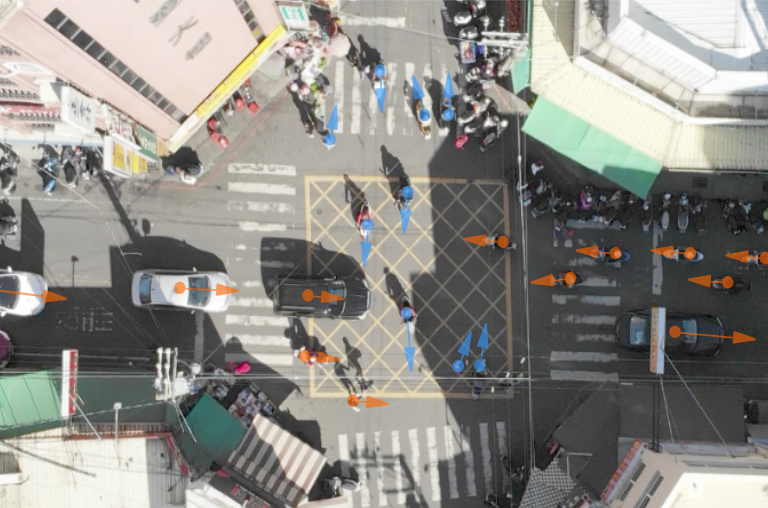
\includegraphics[scale=0.5]{complex_intersection_mod_demo.png}
\end{center}
\caption{A crossroad with no signal.}
\label{INTERSECTION} 
\end{figure}

Typical urban scenarios such as merging into lanes, entering roundabouts and crossing over  crossroads with no signals, all require various ways to interact with surrounding agents. For example, in Fig.~\ref{INTERSECTION} we show an unsignalized crossroad in central Taiwan. Arrows represent the velocity vectors of the vehicles in this scene. Interactions among traffic participants are based on their perception of others' intentions, and their capability in presenting their own. Method used to realize the intentions of others together with the method to show intentions of oneself are both urgently required.



%%%%%%%%%%%%%%%%%%%%%%%%%%%%%%%%%%%%%%%%%%%%%%%%%%%%%%%%%%%%%%%%%%%%%%%%%

%{ motion planning }
\section{LITERATURE REVIEW}
Techniques for autonomous vehicles in motion planning have been studied extensively in recent years \cite{motion_planning}. Various algorithms are developed for optimized and collision-free trajectories. However, these algorithms tends to assume the future trajectories of other agents to be known, while in fact we have only limited knowledge about how other surrounding vehicles will behave. Without in-traffic direct communications or high-level traffic commands, this over-simplified assumption will result in unrealistic and often over-cautious reaction to avoid collisions.

%{ classification of motion models }
Predicting surrounding vehicles' movements enables more active and more practical traffic studies. In the literature, physics-based motion predictions use dynamic or kinematic models governed by simple physics laws as surveyed in \cite{survey_motion_prediction}. These models requires less computational power, easier to construct, and also have decent accuracy in short-term predictions\cite{physics_real_time, physics_velocity_obstacle}. Nevertheless, the original functions do not account for uncertainties in real traffic, as a result, have only limited ability to interact with other human drivers. Zhan et al. use  probability model of yielding/passing actions at a crossroad in the traffic optimization study in \cite{non-conservative}.

Other prediction models such as the work of Zhan et al. and Ruf et al. \cite{sparc} use a cost map with probabilistic values on each path to optimize the global planner of vehicle movements. In spite of better long-term prediction, the interaction with surrounding participants is still not considered.

In order to generate interactive models, probabilistic methods such as partially observable Markov decision process (POMDP) have been applied.  POMDP can decide the actions of the host agent while interacting with other traffic participants by predicting their future states and taking their current state into account. Navigation and obstacle avoidance are solved in a probabilistic manner using POMDP by Foka et al. \cite{Foka}. Hubmann et al. \cite{state_uncertain_environment} also use POMDP to evaluate the possible maneuvers of other agents and optimize the actions of the host agent. Despite the advantages, POMDP is typically solved off-line, which means it's intractable for large state spaces. Hence, to avoid the complexity, the problems are often simplified.

%{freezing robot problem}
Even though these motion models consider the interaction with other traffic participants and generate the optimized action, the explicit interactions that we use for more realistic scenarios such as entering a round about or crossing a crossroad are still not included. Both the presentation of social behavior by human driven vehicles or the situations that need autonomous vehicles to react to are vital to the mixed fleet problem. 

 Autonomous devices are expected to share the environment with people, therefore the capability for them navigating in natural world without collisions is indispensable. However, as illustrated in \cite{trautman}, since the uncertainty explosion in future state, the “Freezing Robot Problem” (FRP) occurs when navigating through cluttered and dynamic environment with over conservative strategies. The authors also show that the FRP will still happen even under perfect prediction of other agents. This is potentially solvable if we enable the autonomous vehicle the ability to "create the dominance by making a move".

%{autonomous vehicle can influence human drivers’ decision}

Sadigh et al. \cite{leverage} proposed a method applying Inverse Reinforcement Learning to acquire approximated human reward function from human driver demonstrations, which was latter used to demonstrate that the actions of the autonomous vehicle can affect those of the human. The result suggests that the freezing robot problem, which was due to over defensive action of autonomous vehicle, could be alleviated, if we know how certain action is reacted to.

The main focus of this work is first to define a probabilistic model that can perceive the intentions of other drivers in urban environments which can be an input for the motion planning of autonomous vehicles in the future. In order to be capable of reading human drivers' behaviors, in Section 3, we start from modeling the unsignaled crossroads that require communication between participants to take safe and applicable actions. Probability of time to collision (TTC) and time to action (TTA) are introduced using the concept of critical warning distance. Our models are validated in Section 4 via several real-world crossroad scenarios. Section 5 provides the discussions and conclusions.

%%%%%%%%%%%%%%%%%%%%%%%%%%%%%%%%%%%%%%%%%%%%%%%%%%%%%%%%%%%%%%%%%%%%%%%%
\section{CROSSROADS MODELING}

When crossing an unsignalized crossroad, the longitudinal speed is decided empirically by human. We observe the oncoming vehicle in a short amount of time and estimate the next possible position, speed and direction the vehicle might be, mostly by experience. We then adjust our speed accordingly: pass the vehicle if we \textbf{believe} we can arrive at the crossroad before the opponent, or yield if we can't. Since we don't perceive the world numerically, many researchers have suggested that the time to hit an object for different observers could be estimated\cite{cog}. A probabilistic model of driving behavior is then developed.

 Figure \ref{model_demo} illustrates a human driver (on the left, heading to the right) and an autonomous vehicle (on the bottom heading upward) crossing a perpendicular crossroad with no signal. In this scenario, to reduce the dimensionality of the state space, we focus only on the longitudinal states of both vehicles with their extended line of movement intersect each other at  \textbf{\emph {the node}}, we use symbol $\oplus$ to represent it in the following paper. $\oplus$ is used as the origin of the coordinate system. The positive $x$ direction is same as the vector of velocity of the first approaching vehicle, and positive $y$ direction as the vector of velocity of the other vehicle. The state of ego vehicle is defined as : 
\begin{equation}
\mathbf{S_i} = \Biggl( \begin{array}{c} \mathbf{d_{node,i}} \\ \mathbf{v_i} \\ \mathbf{a_i} \end{array} \Biggr), \mbox{ where }  i=\{a, h\} 
\label{sa}
\end{equation}
$d_{node, i}$ is the displacement from the position of the vehicle to that of $\oplus$, while $v_i$ and $a_i$ are the the speed and the acceleration of autonomous vehicle ($i=a$) , and of human driver ($i=h$), respectively . Note that they are both one-dimensional. 
%Similarly, the state of the human driving vehicle is:\\

% \begin{equation}
% S_h = \Biggl( \begin{array}{c} l_h \\ v_h \end{array}  \Biggr)
% \label{sh}
% \end{equation}


\begin{figure}[t]
\begin{center}
%\setlength{\unitlength}{0.012500in}
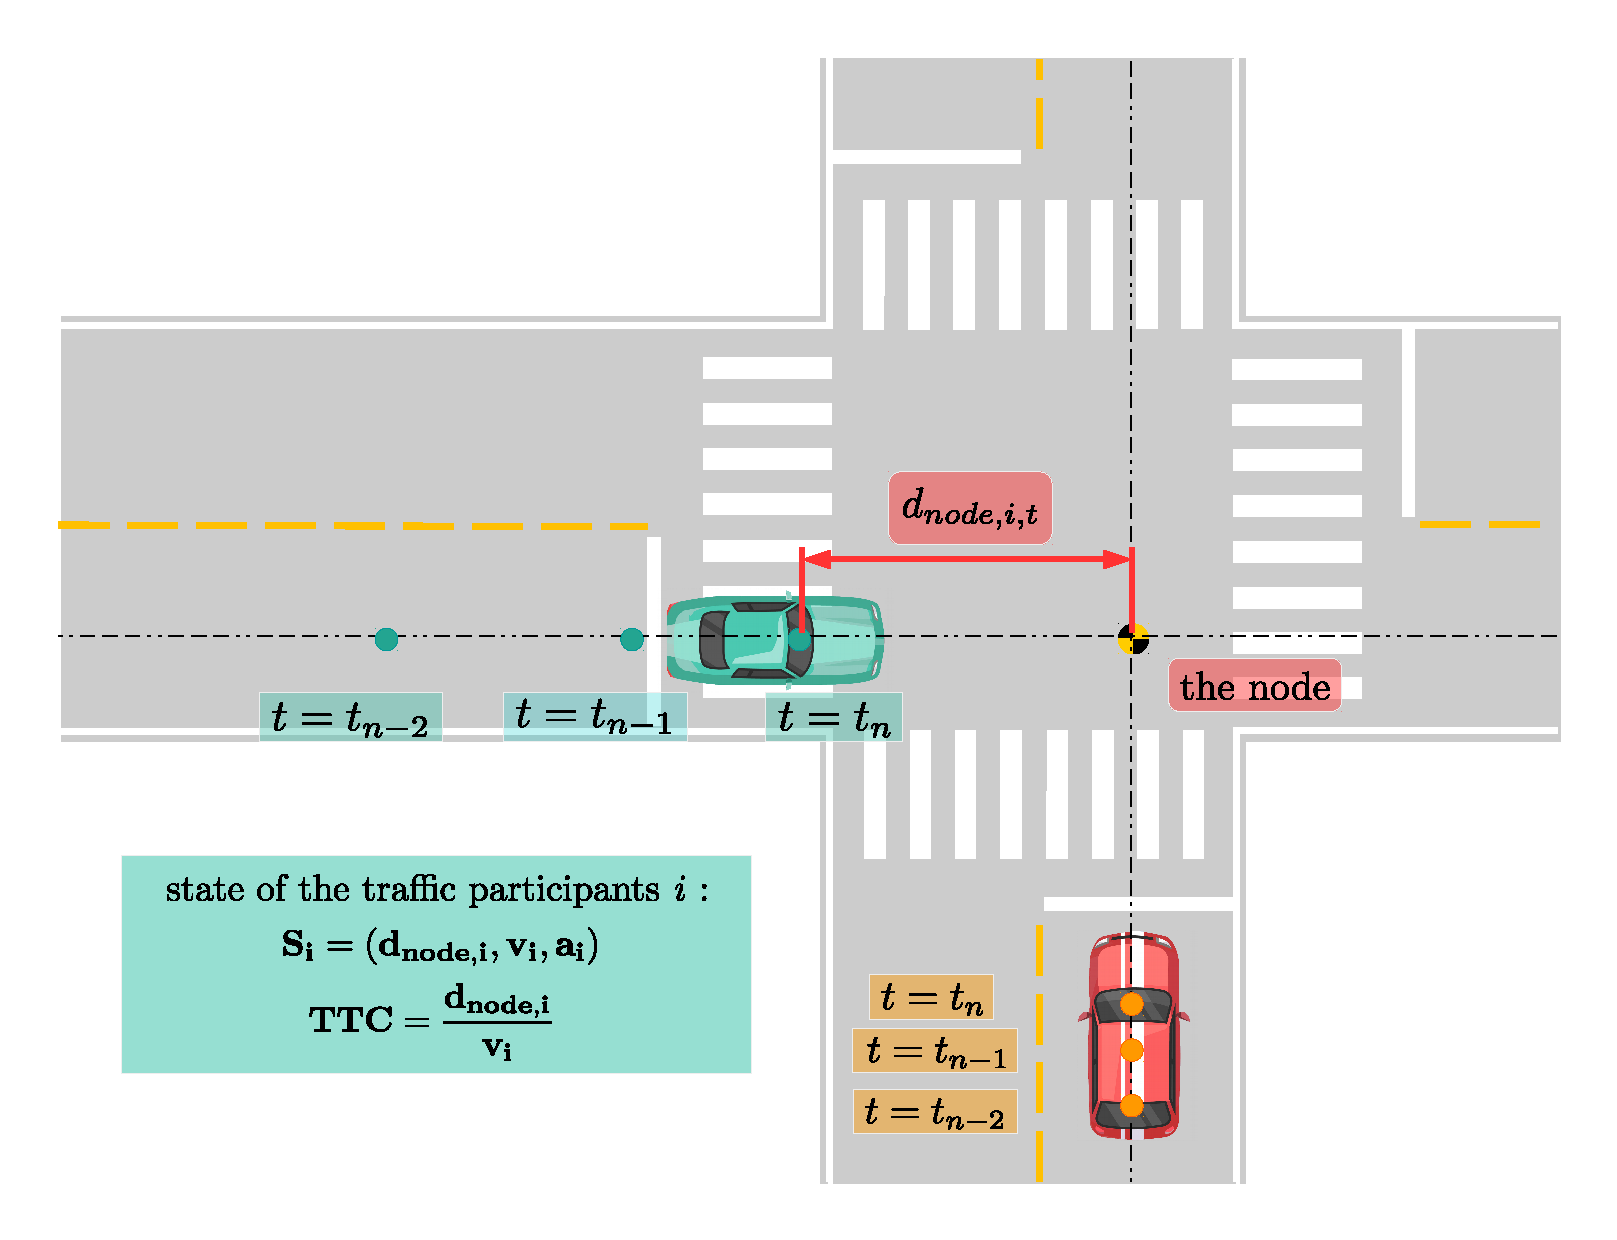
\includegraphics[scale=0.3]{intersection_concept.pdf}
\end{center}
\caption{Demonstration of the proposed scenario and relevant variables.}
\label{model_demo} 
\end{figure}


%%%%%%%%%%%%%%%%%##################%%%%%%%%%%%%%%%%%%%%%%%%%%%%%%%%%
\subsection{Time to Collision and Time to Action}


Before we continue explaining the proposed method, we are going to briefly introduce the concept of Time to Collision (TTC). Also known as time to contact, TTC represents the time it will take to reach the obstacle \cite{TTC} if the courses and both speeds are maintained. This approach is widely used as safety indicator. The original definition was specified by an optic variable $\tau_{optic}$ for the "Inverse of the rate of dilation of the target's image on the retina". However, there are intense disputations over whether $\tau_{optic}$ provides necessary TTC information, since both empirical results and analyses suggest that the hypothesis is false \cite{tau}. In this research, we adopted the definition using the speed and the distance from the target in the work of Cavallo et al. \cite{TTC}.

\begin{equation}
TTC = \frac{\text{distance to obstacle}}{\text{speed}}
\label{TTC_2}
\end{equation}


We can then use the definition of TTC to explain how the braking decision is made : under a given speed, the driver decides to brake to avoid collisions when a certain distance is left between the car and the obstacle. As shown in Fig.~\ref{example_TTC_TTA}, a car is approaching from the left and a red obstacle is on its path. At point $P_A$, the car is cruising with constant speed $V_0$. After the brake being applied at $P_B$, the car begins to slow down and finally comes to a stop with the speed equals to $0$ at point $P_C$. In this scenario, TTC decreases as the distance to the obstacle is getting shorter. Finally at point $P_B$, the driver decides to brake to keep a safe margin from the vehicle to the obstacle when the car is fully stopped. The distance from point $P_B$ to the obstacle is the "distance left before action", which is the minimum distance required to stop in front of the obstacle and keep the safe margin in between. We divide this distance to the speed at the moment and call it Time to Action (TTA). TTA then stands for the threshold TTC that the driver decide to take action (brake) to avoid collision.  


\begin{figure}[htbp!]
\begin{center}
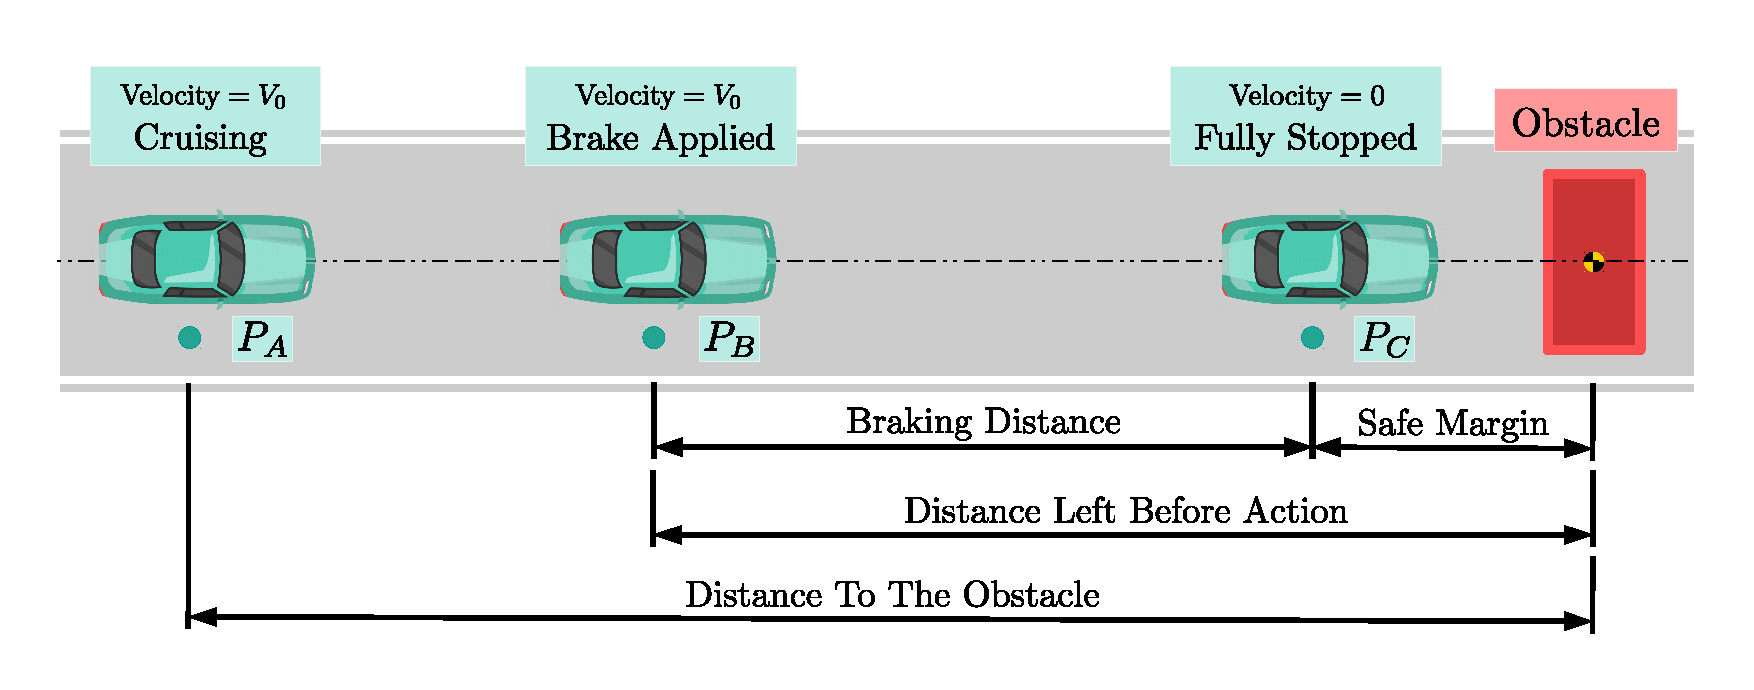
\includegraphics[scale=0.3]{example_TTA_TTC.pdf}
\end{center}
\caption{Illustrations of TTC and TTA.}
\label{example_TTC_TTA} 
\end{figure}


The time-history of TTC and the dependent variables depicted in Fig.~\ref{example_TTC_TTA} are presented in Fig.~\ref{TTC_history},which is similar to the time-history of braking in the work of Winsum et al. \cite{time_history}. As the vehicle cruises from point $P_A$ to $P_B$ in Fig.~\ref{example_TTC_TTA}, in Fig.~\ref{TTC_history} the TTC drops from $t=0$ to $t=t_0$. Then, the driver brakes at point $P_B$ in Fig.~\ref{example_TTC_TTA}, where in Fig.~\ref{TTC_history} the driver brakes at time $t_0$ and the TTC value equals to TTA of the driver under this speed. The driver brakes at this TTC since he or she believes that a collision would happen if it is applied any later. During the braking, TTC drops to its lowest point labeled as TTC min and then rises. The rise is due to the the speed decreasing rate being higher than the rate of the distance decrease. Note the TTA is the minimum TTC that drivers start to hit the brake to avoid collision, not the minimum TTC during the whole process (which is the TTC min).


\begin{figure}[htbp!]
\begin{center}
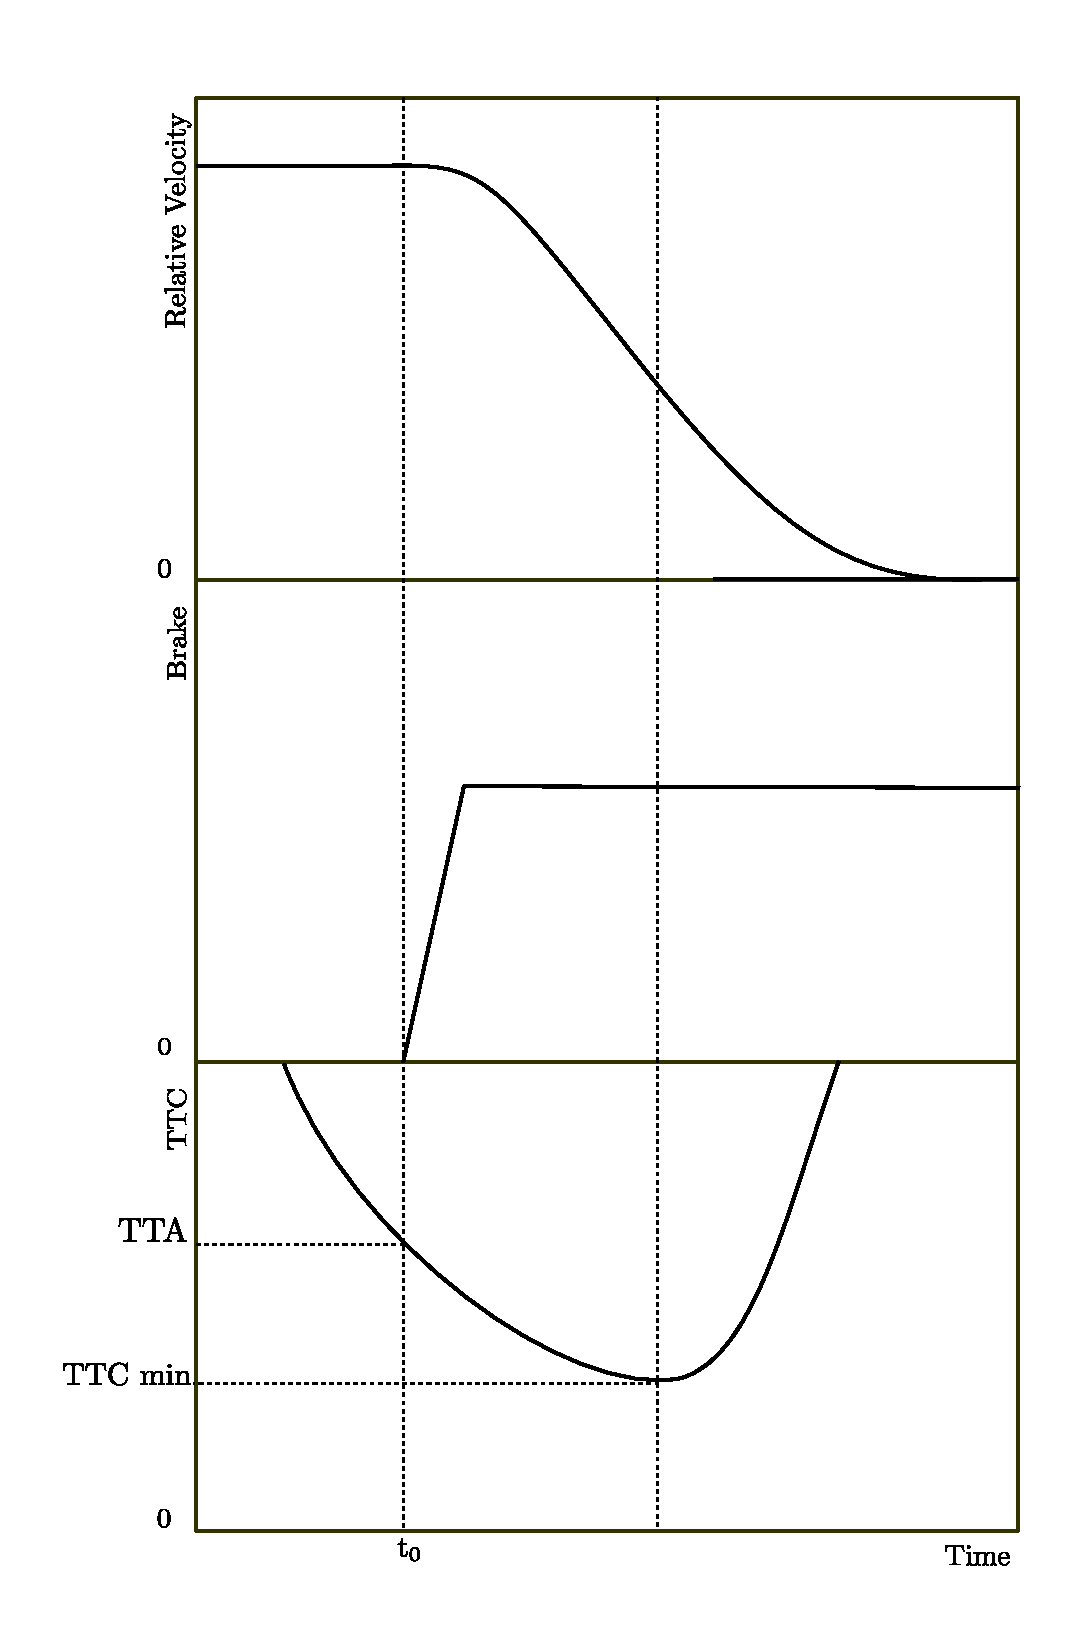
\includegraphics[scale=0.4]{TTC_change_when_braking.pdf}
\end{center}
\caption{History of time to collision when brake is applied.}
\label{TTC_history} 
\end{figure}


Now we bring TTC and TTA into our crossroads scenario. From the above we know that people can not directly decide the braking timing from speed and distance. Instead, we decide when to brake with the help of TTC that we learn from visual cues. Similarly in the crossroad scenario, when a vehicle is about to arrive at the crossroad at the same time as the host vehicle, the driver of the host vehicle will brake when the learned TTC is equivalent to his TTA to avoid potential collision. Note that in this scenario, the obstacle to avoid is the potential collision at $\oplus$ (the intersect of two routes). If we can find out this TTA that the driver start to take action, we can know around which time it is highly possible that the driver will hit the brake and stop.



%%%%%%%%%%%%%%%%%##################%%%%%%%%%%%%%%%%%%%%%%%%%%%%%%%
\subsection{Distribution of TTA and Probability Density Function}

From the above paragraph, we know that the definition of TTA is the minimum TTC (or the minimum distance left before braking at the current speed) that drivers start to hit the brake to avoid potential collision. In fact, TTA differs from person to person since each of us has our own risk threshold to decide when to hit the brake. For example, a young driver with a high performance sports car might have a relatively low TTA because of his personality and the great braking performance of the car allowed the driver to go closer before braking. On the contrary, an older driver driving an aged passenger sedan might have a higher TTA since the driver is more cautious and the car requires longer distance to stop.

In Fig.\ref{TTC_TTA} we use the grey area to illustrate the distribution of TTA among general people (95\% of people's TTAs are within the area) and solid line as the TTC of host agent. The distribution of TTA can be explained as "at this range of TTC, 95\% of drivers will start the action (hit the brake)". If we see the TTC of a driver is getting lower, when the value reaches the mean value of the TTA among general people, we can say that there is 50\% chance that this driver will brake at this very TTC. Furthermore, by assuming the distribution is normally distributed, we can have Fig.~\ref{TTC_distribution} representing the probability density function of general people's TTA and use this to calculate the corresponding probability. For example, in Fig.~\ref{TTC_TTA} the solid line indicating the TTC of the host agent change with time. As the TTC drops below 5.5 seconds, we can get the probability of the driver to apply the brake is 0.0668 by integrating the probability density function in Fig.~\ref{TTC_distribution} from the corresponding TTC to +inf.

What should be noted here is that since whether the driver brakes or not, the distance to $\oplus$ during that time is always decreasing. Hence the value of TTC will either start to rise eventually or remain the same  when the brake is applied and the vehicle is about to stop. The TTC used to calculate the probability is hence the lowest TTC that occurs in the TTC curve of the host agent. We will use Fig.~\ref{TTC_TTA} and ~\ref{TTC_distribution} to further explain this idea. 

In Fig.~\ref{TTC_TTA}, the dashed lines indicated by colored triangles on both sides represent some moments during the process. The red indicated is at 2.5 seconds on the time line, the blue at around 5.5 seconds and the magenta at around 7 seconds. The corresponding moments are also labeled on the TTA distribution in Fig.~\ref{TTC_distribution}. At 3 seconds (red indicated line, red line in short) the TTC of the host agent is around 5.6 seconds, from the distribution we know that the probability of the vehicle stopping is 0.0548, which is the area right side of the red line. Similarly, when the time is at 5.6 seconds (blue line), the probability of the vehicle stops rise to 0.46. As it comes to the time at 7 seconds (magenta line) the TTC becomes larger than the previous time, but as mentioned before, the rising of TTC indicates the agent is slowing down, which does not lower the probability of stopping. So the probability of the host agent stopping is still calculated using the lowest TTC value as used earlier which is 0.46.

\begin{figure}[htbp!]
\begin{center}
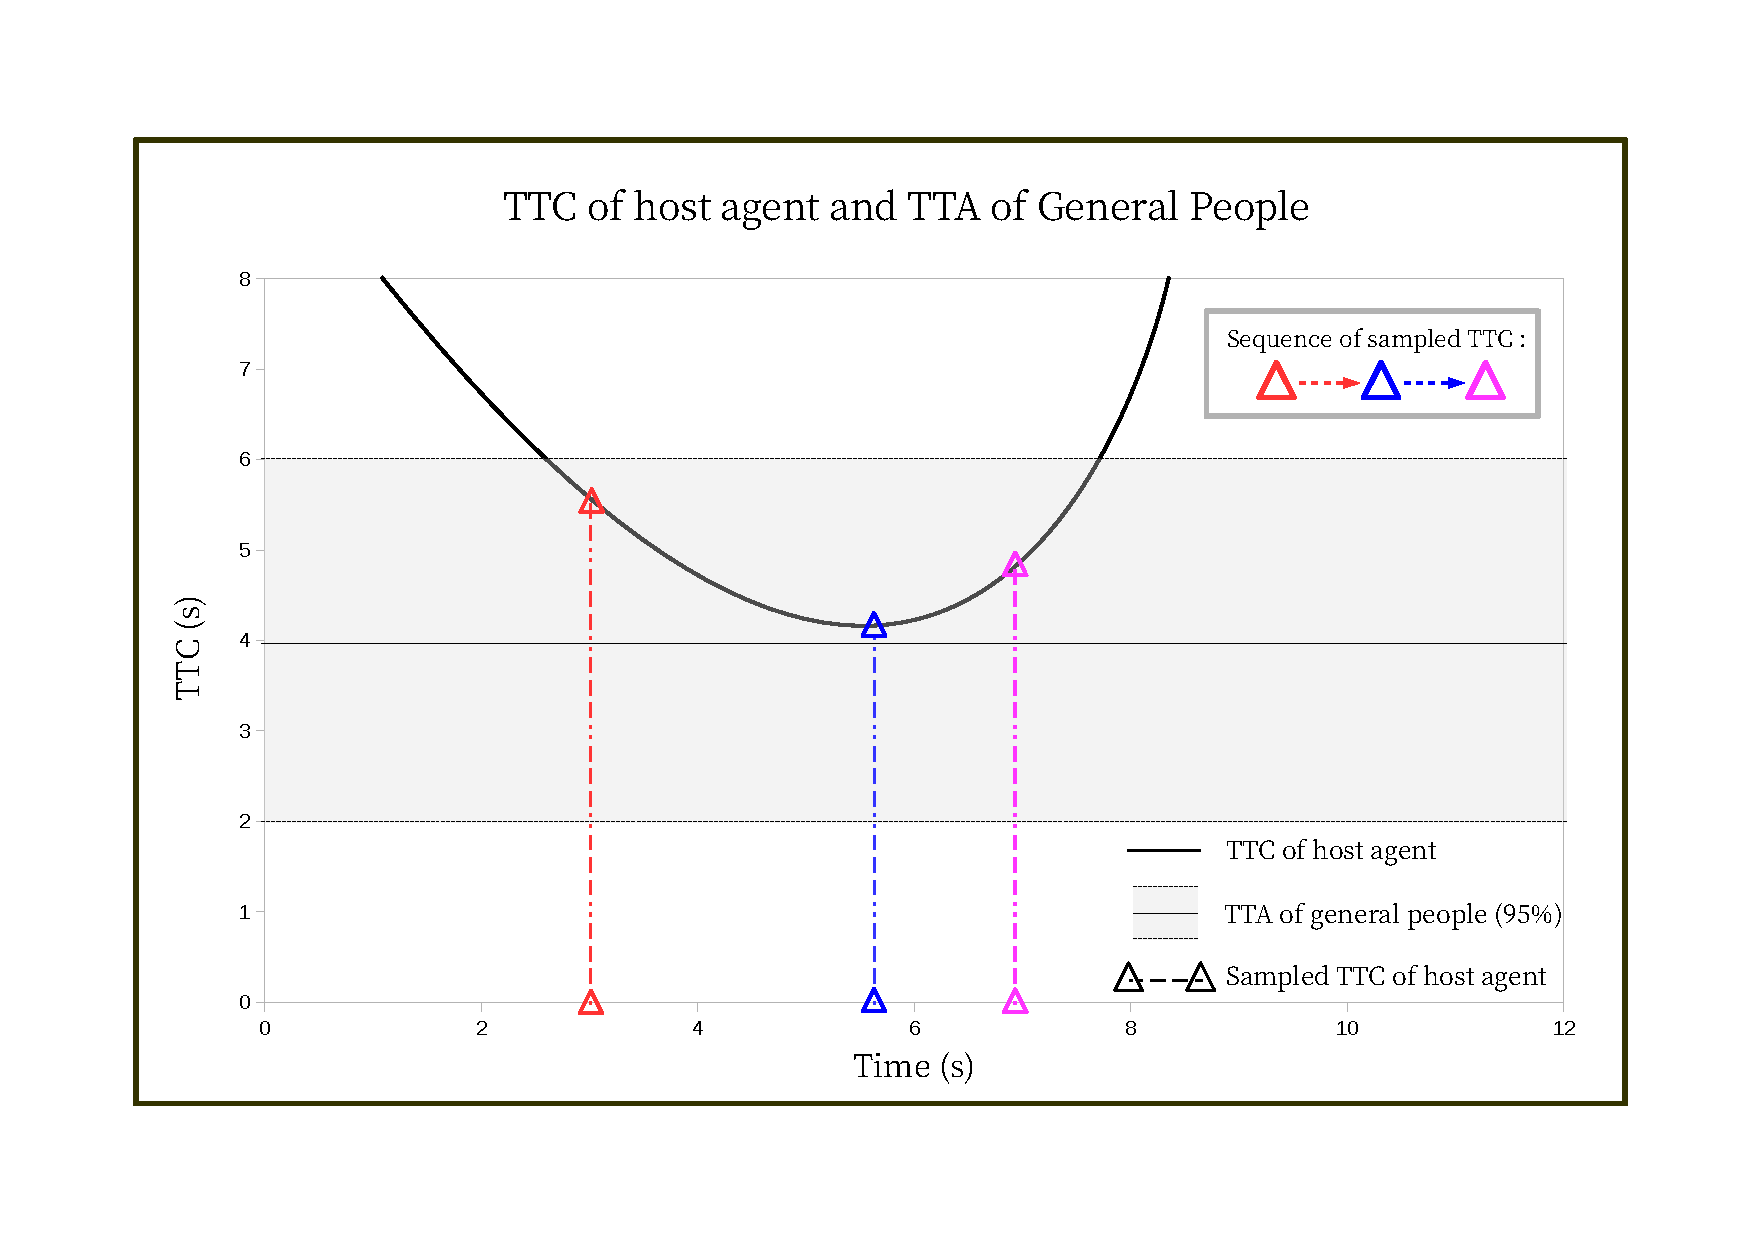
\includegraphics[scale=0.31]{TTC_probability.pdf}
\end{center}
\caption{Example of TTA among general people and TTC of the host agent.}
\label{TTC_TTA} 
\end{figure}

\begin{figure}[htbp!]
\begin{center}
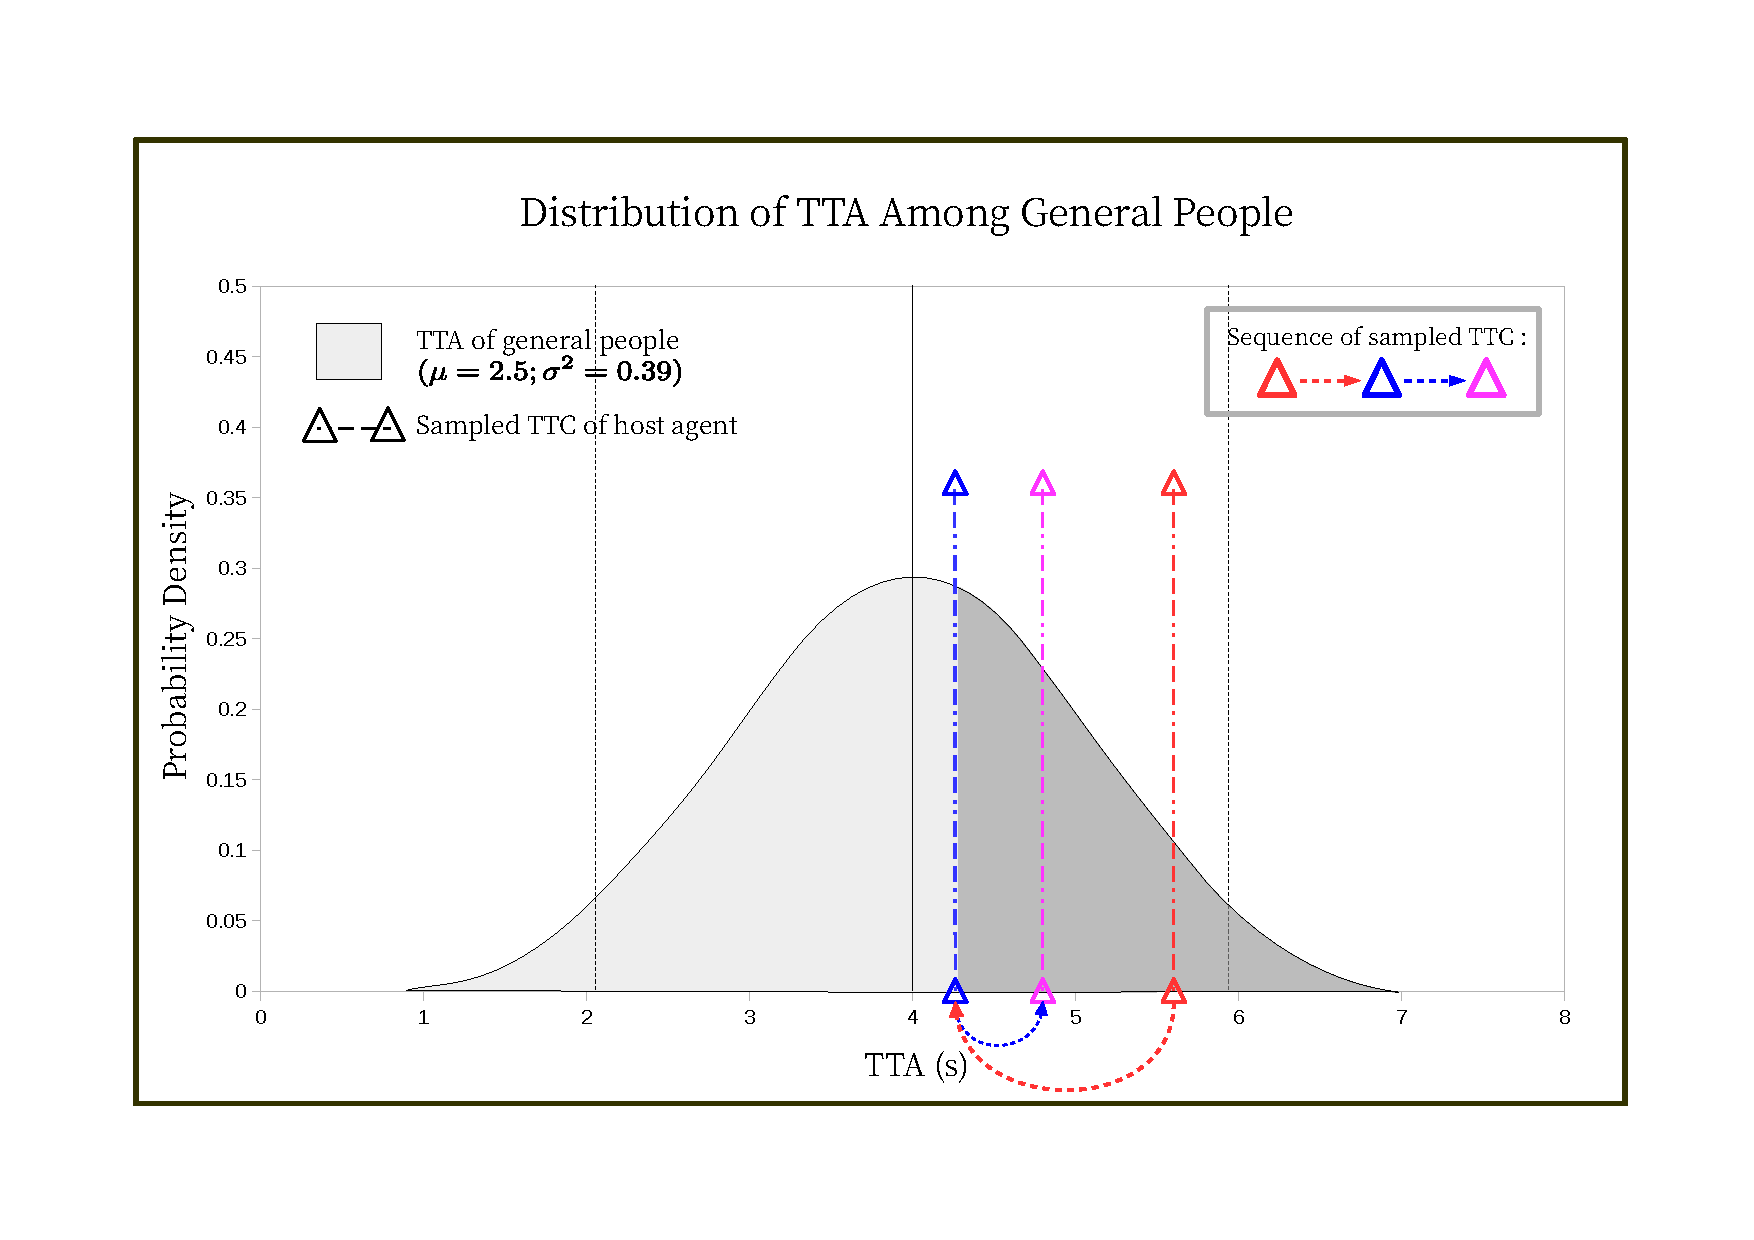
\includegraphics[scale=0.31]{TTC_probability_distribution.pdf}
\end{center}
\caption{Example of TTA distribution among general people.}
\label{TTC_distribution} 
\end{figure}

%%%%%%%%%%%%%%%%%##################%%%%%%%%%%%%%%%%%%%%%%%%%%%%%%%
\subsection{Probability of Stopping}

However, using solely the TTC to find the probability of stopping in TTA distribution is not thorough enough. For example, situations like a driver who drives towards $\oplus$ without decelerating will result in a decreasing TTC curve and a rising probability of stopping (the area on the right side of TTA distribution increases). To take situations like this into account, a weighting parameter is needed. Next, the model describing driver behaviors is introduced and the weighting parameter is defined afterwards.

In this work, we focus on the crossroad scenario described earlier in which drivers drive toward $\oplus$ (the intersection of courses). Since $\oplus$ is the point for a potential collision, we then use the displacement from the vehicle to $\oplus$ as the distance to obstacle in Eqn.~(\ref{TTC_2}). Here we have the displacement from vehicles to $\oplus$ as $d_{node,i,t}$ with $i \in \left\{ {a, h}\right\}$ for autonomous vehicle and human driver separately and $t$ is the time step. After that, we approximate it by assuming the acceleration is constant in every time step:

\begin{equation}
d_{node, i, t} = d_{node,i,0} - \biggl(v_0t+\frac{1}{2}at^2\biggr)
\label{d_node}
\end{equation}

Where $d_{node,i,0}$ is the initial displacement from the vehicle to $\oplus$, $v_0$ is the initial speed and $a$ the acceleration applied. Then, the TTC of the vehicle is described as :

\begin{equation}
TTC = \frac{d_{node,i,t}}{v_t}
\label{TTC_3}
\end{equation}

The $v_t$ in the equation is the velocity at that moment. Now we need a weighting parameter to solved the problem explained at the beginning of this subsection. 

The weighting parameter is required, because the probability we get by integrating the probability density function based on the given TTC alone can not distinguish the stopping from all the other states of the vehicle. For example, as described in Fig.~\ref{TTC_acc}, a vehicle is accelerating through $\oplus$, resulting in the increase of the integrated stopping probability as it approaches $\oplus$, due to the decrease of the TTC. The vehicle, however, has no intention of stopping, which suggests that the using TTC alone is not enough to indicate the chance of stopping. Similar result could be seen, as a vehicle starts to brake far away from $\oplus$ and the integrated stopping probability remains low, because of the high TTC.


\begin{figure}[htbp!]
\begin{center}
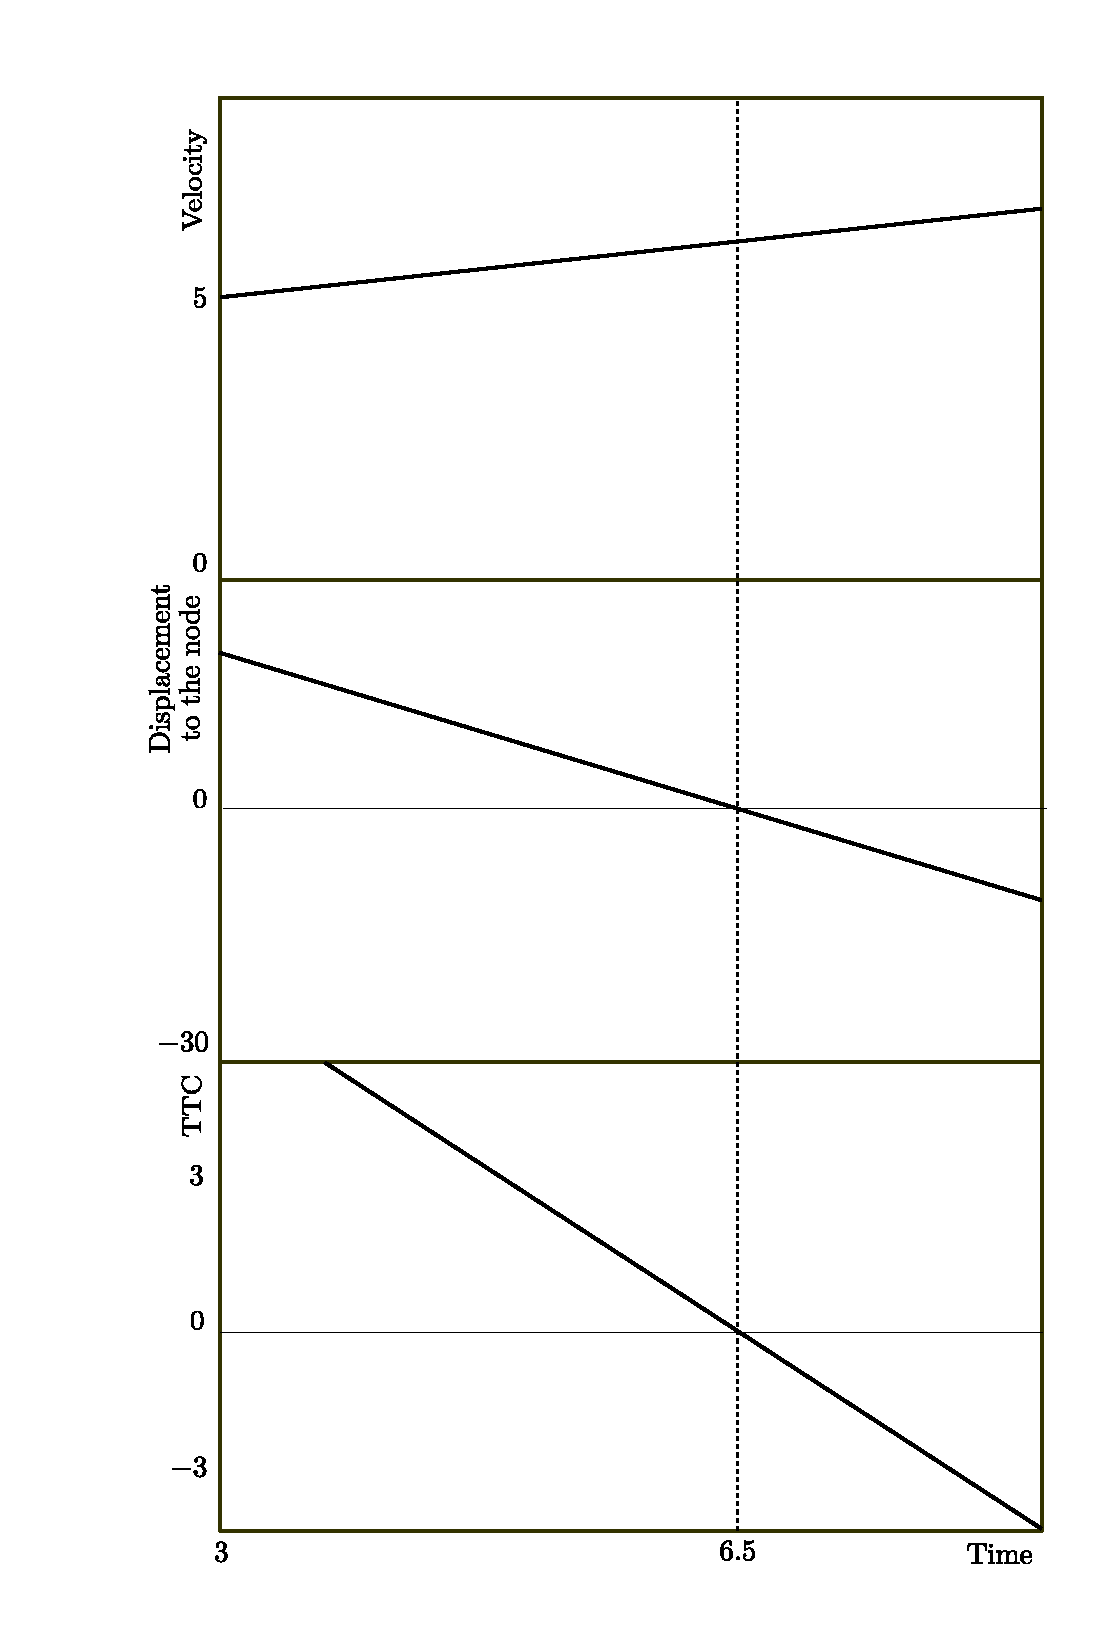
\includegraphics[scale=0.43]{TTC_change_when_accelerating.pdf}
\end{center}
\caption{History of TTC as the vehicle accelerating through $\oplus$.}
\label{TTC_acc} 
\end{figure}

To conclude, the weighting parameter should be capable of punishing those with low TTC while accelerating or at high speed and rewarding those with deceleration or low speed. So we choose the derivative of TTC as the element of the weighting parameter since it can take both the speed and the acceleration into consideration at the same time.

From Eqn.~(\ref{d_node}) and (\ref{TTC_3}), the derivative of TTC is :

\begin{equation}
TTC' = \frac{d}{dt}\frac{d_{node,i,t}}{v_t} = -1 -a \cdot d_{node,i,t} \cdot v_t^{-2}
\label{TTC'}
\end{equation}

To make the the weighting consistent to what we suggested earlier, conditions and the reward ratio $\alpha$ are used. we call this final form of weighting parameter $\gamma$.

\begin{equation}
    \gamma = 
    \begin{cases} 
     0 &~~\text{if}~~TTC' + 1<0\\
    \big(TTC' + 1\big)\times \alpha &~~\text{if}~~TTC' + 1>0\\
    -1 &~~\text{otherwise}
    \end{cases}
\label{gamma}
\end{equation}

We can see from Eqn.~(\ref{TTC'}) that if the vehicle slows down, meaning that $a<0$, the value of TTC' will become greater than -1 since both $d_{node,i,t}$ and $v_t^{-2}$ are greater than 0. Substitute TTC' into Eqn.~(\ref{gamma}) we have the gamma that increase linearly with TTC'. Similarly, when the vehicle is speeding up, meaning that $a>0$, which results in TTC' smaller than -1. Same as the last condition, substitute the TTC' into Eqn.~(\ref{gamma}) again, the value becomes 0. Finally, the weighting parameter is multiplied by the probability we integrated.

\begin{equation}
    P_{stop} = 
    \begin{cases} 
    1&~~\text{if}~~\Bigr(1-\Phi\big(min TTC\big)\Bigl) \cdot \gamma > 1\\
    1&~~\text{if}~~\gamma = -1\\
    \Bigr(1-\Phi\big(min TTC\big)\Bigl)\cdot \gamma &~~\text{otherwise}    
    \end{cases}
\label{p_stop}
\end{equation}

The $\Phi$ here is the cumulative distribution function of general people's TTA which can be acquired by integrating the probability density function similar in Fig.~\ref{TTC_distribution}. The $minTTC$ here is the lowest TTC during the interaction as described in Fig.~\ref{TTC_TTA} and \ref{TTC_distribution}.

Among vehicles decelerating in different degree, the use of TTC' in $\gamma$  not only gives the method the ability to determine how drastically the vehicle is stopping, but it also helps the method to decide whether this car is actually going to stop or just crossing over when a relatively low TTC is reached. So when a vehicle is sliding through $\oplus$ ($a = 0$), despite the TTC is getting smaller and results in higher probability, the value of $\gamma$ at this instance is 0 since TTC' equals to -1, and that make the probability of stopping 0. Similarly, the value of $\gamma$ is also 0 when the vehicle is accelerating toward $\oplus$. As for the cases that the vehicle is braking, the value of $\gamma$ varies from 0 to $\alpha$ which gives proportional reward to different degrees of braking applied, e.g. when the brake is applied, larger values of deceleration (harder the brake is stepped) is rewarded with larger $\gamma$, which increases the probability of the vehicle stopping.

Now the remaining problem is how to acquire the probability density function of TTA among average people. Since the research concerning this topic is not available, a relatively indirect estimation method is used. To begin with, the "perfect TTA" should be estimated. We reference algorithms that determine critical warning distance \cite{CWD} and come up with the estimated TTA:

\begin{equation}
TTA_{est} = \frac{R_i+v_i\tau+R_{min}}{v_i} 
\label{TTA_est}
\end{equation}

Where $v_i$ is the speed of target vehicle, $\tau$ represents the reaction time needed and $R_{min}$ is the minimum range left between target vehicle and $\oplus$ when it's fully stopped.
Where $R_i$ is the stopping distance of target vehicle $i$ with equation:
 
\begin{equation}
R_{i} = \frac{v_i^2}{2a_{dec}}
\label{R_i}
\end{equation}

The value of $a_{dec}$ in Eqn.~(\ref{R_i}) is the deceleration rate. Values of $\tau$, $R_{min}$ and $a_{dec}$ are 0.6 seconds, 5 meter and 6 $m/s^2$ respectively as suggested by the Mazda Algorithm in the literature. 

Note that the values of $\tau$ and $R_{min}$ could be used as the parameters related to driving patterns, e.g. the young guy driving a Porsche might have a smaller $\tau$ since in average the reaction time is shorter among younger groups and the $R_{min}$ is also smaller due to the excellent performance of the car. Using these parameters, the $TTA_{est}$ can then represent the minimum time left for the driver to take action (braking) and prevent collision from happening.

In the work of Cavallo et al. \cite{TTC}, the on-road experiments are conducted to find out the accuracy of the estimation of TTC among different groups of people and different visual conditions. Results of this literature suggested that relationships between actual and estimated TTC could be expressed as $y = 0.73x+0.04$ and $y=0.57x+0.15$ for experienced driver and beginners respectively. Where in the equations the x-axis is the actual TTC and the y-axis is the estimated TTC. The error magnitude, on the other hand, at around 28\% for experienced drivers and 47\% for beginners. To apply this result to general people, mean values of estimation error of experienced and beginner drivers are used: 
\begin{equation}
y = 0.65x+0.15
\label{TTA_mean}
\end{equation}

The error of this regression is 37.5\%.

As mentioned earlier, the estimated TTA that stands for the minimum time left to action so as to avoid collision, can correspond to the estimated TTC in the equations since both of them are perceived by us. We substitute the estimated TTA as $y$ into the approximated function and acquire the actual TTA. The actual TTA is then used as the mean value of the TTA distribution and 37.5\% of this value as two standard deviations.

So far we used the specific TTC called TTA to define the minimum time left for drivers to hit the brake before the the collision happens. A novel method is proposed to estimate the probability of the vehicle stopping using the TTA distribution and the derivative of TTC. Finally, approximated distribution of TTA is found using the concept of critical warning distance.

%%%%%%%%%%%%%%%%%%%%%%%%%%%%%%%%%%%%%%%%%%%%%%%%%%%%%%%%%%%%%%%%%%%%%%%%%%%
\section{VALIDATIONS AND RESULTS}
In order to confirm and evaluate the similarity between the proposed method and the behavior of human drivers, observation of interaction between two human driven vehicles at a unsignalized crossroads is conducted.

\subsection{Observation Technique}
To collect the related data, the drone for aerial filming is used at the crossroad in urban environment (\textit{Bo’ai Rd.93-85, Yuanlin City, Changhua County 510, Taiwan (23.958606, 120.573283)}). After the observation, we use Tracker, a video analysis tool, to collect and analyze relevant variables e.g. positions and velocities as shown in Fig.~\ref{aerial_filming}. Note that the angle of the road on the left hand side (about $6.7^\circ$) could be ignored since it only results in approximately 0.1\% difference in velocity. Red and cyan circles indicate the position history of the vehicles at that moment, and $\oplus$ is set at the intersect of two courses. Interval between every two frames is 0.042 second (24 fps). With the position and the time, the velocity is calculated. To better evaluate the driving behavior, we choose clips with maneuvers of two vehicles that are likely to cause a collision. 

\begin{figure}[htbp!]
\begin{center}
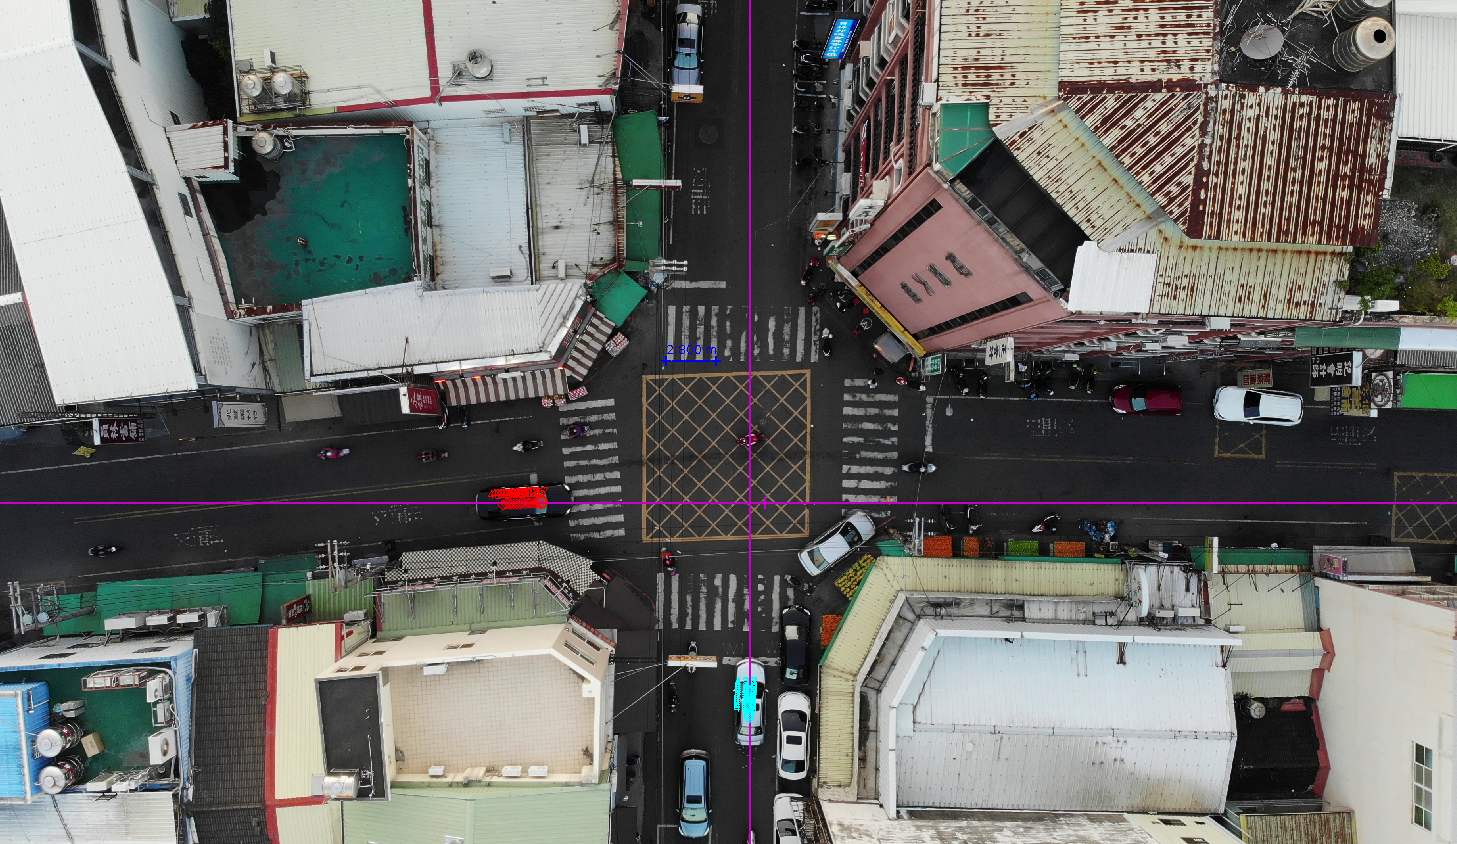
\includegraphics[scale=0.17]{aerial_filming_demo.png}
\end{center}
\caption{Using video analysis tool to track vehicles driven by humans.}
\label{aerial_filming} 
\end{figure}


\subsection{Results and Analyses}

Parameters used in the proposed method are listed in Table~\ref{table_parameters}. All the parameters except $\alpha$ are based on the Mazda Algorithm \cite{CWD} which is used to determine the threshold distance that triggers the Collision Warning System. With validations in literature, we believe the values are generally applicable. As for the reward ratio $\alpha$, with more discussion in the next section, we chose 1.5 here to have higher output probabilities on average for more obvious results. With all parameters and variables needed, the probability of stopping is calculated every 0.5 second.

\begin{table}[t]
\caption{TABLE FOR PARAMETERS USED.}
\begin{center}
\label{table_parameters}
\begin{tabular}{l l l l c}
& & \\ % put some space after the caption
\hline
\textbf{Parameters} &  & & &\textbf{Values} \\
\hline
Deceleration Rate ($a_{dec}$) &  &  & & 6 $m/s^2$  \\
Reaction Time ($\tau$)        &  &  & & 0.6 $s$ \\
Minimum Range ($R_{min}$)     &  &  & & 5 $m$  \\
Reward Ratio ($\alpha$)      &  &  & & 1.5  \\
\hline
\end{tabular}
\end{center}
\end{table}
 
 
 We start the analysis by calculating the corresponding TTC of Car\_0 (in red) and Car\_1 (in cyan), as illustrated in Fig.~\ref{figure_explaination_TTC}. TTCs correspond to $t_A$, $t_B$, $t_C$, $t_D$ and $t_E$ are shown in the chart of the figure. Afterward, the probability of stopping for each car is calculated using the proposed method and is plotted together with the velocity and the displacement in two separate figures, as illustrated in Fig.~\ref{figure_explaination_1}. We then analyze how the probability of stopping can give assistance to the traffic participants using these figures.
 
 
\begin{figure}[htbp!]
    \centering
    \subfloat[Illustration of calculated TTC of each vehicle.]
    {
    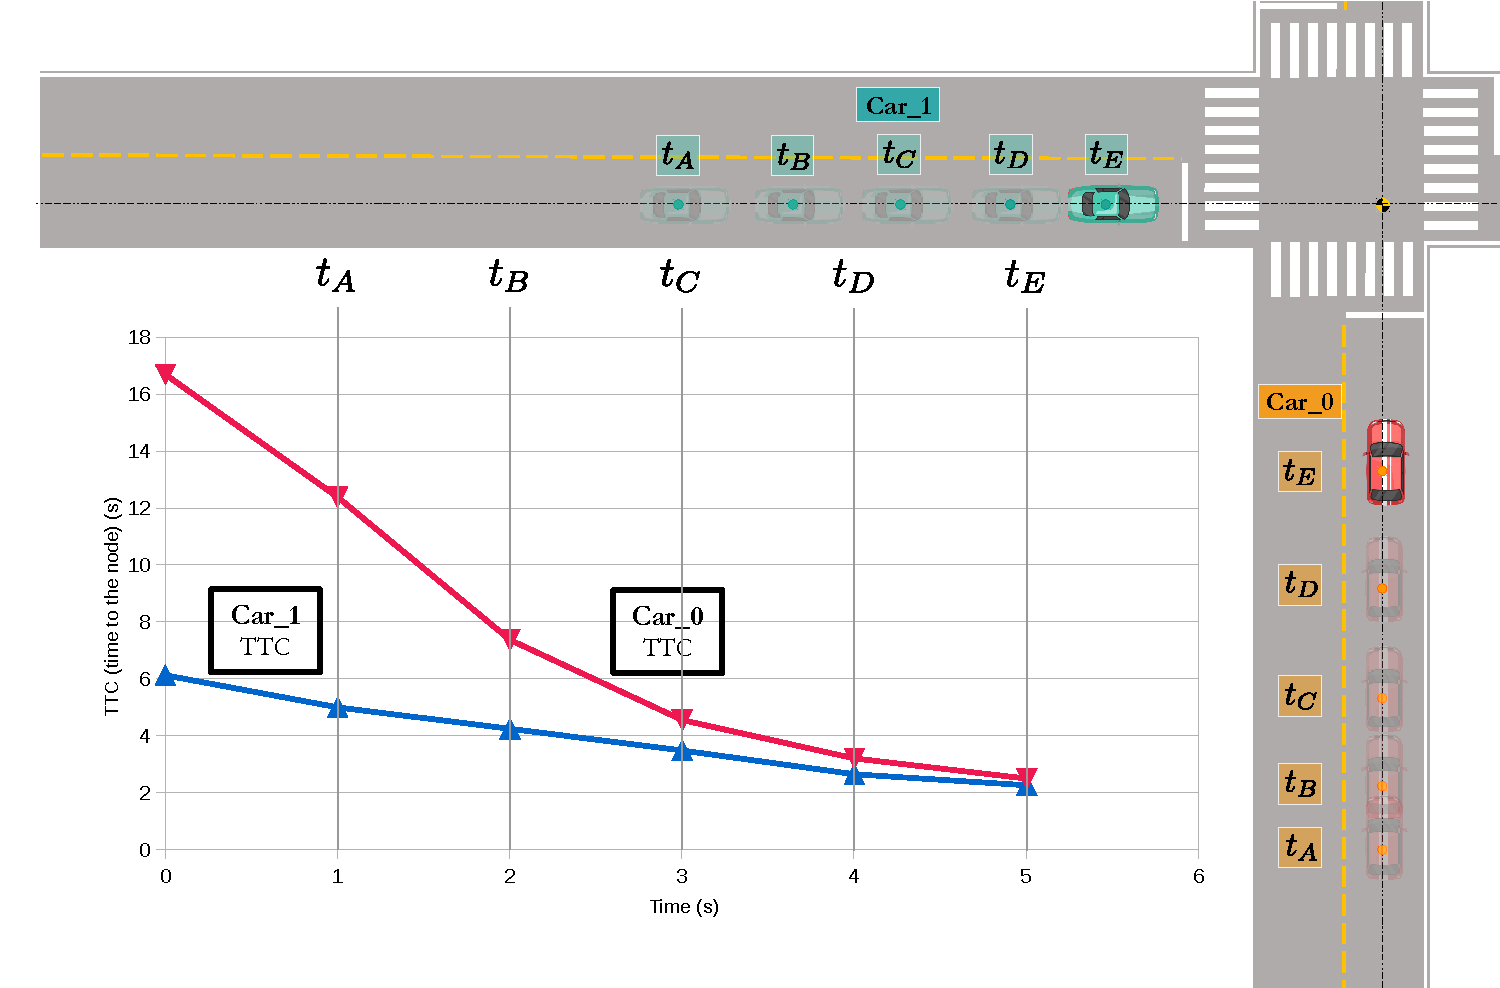
\includegraphics[width=0.4\textwidth]{figure_explaination_TTC.pdf}
    \label{figure_explaination_TTC}
    }\hfill
    \subfloat[Illustration of probability of stopping together with velocity and displacement.]
    {
    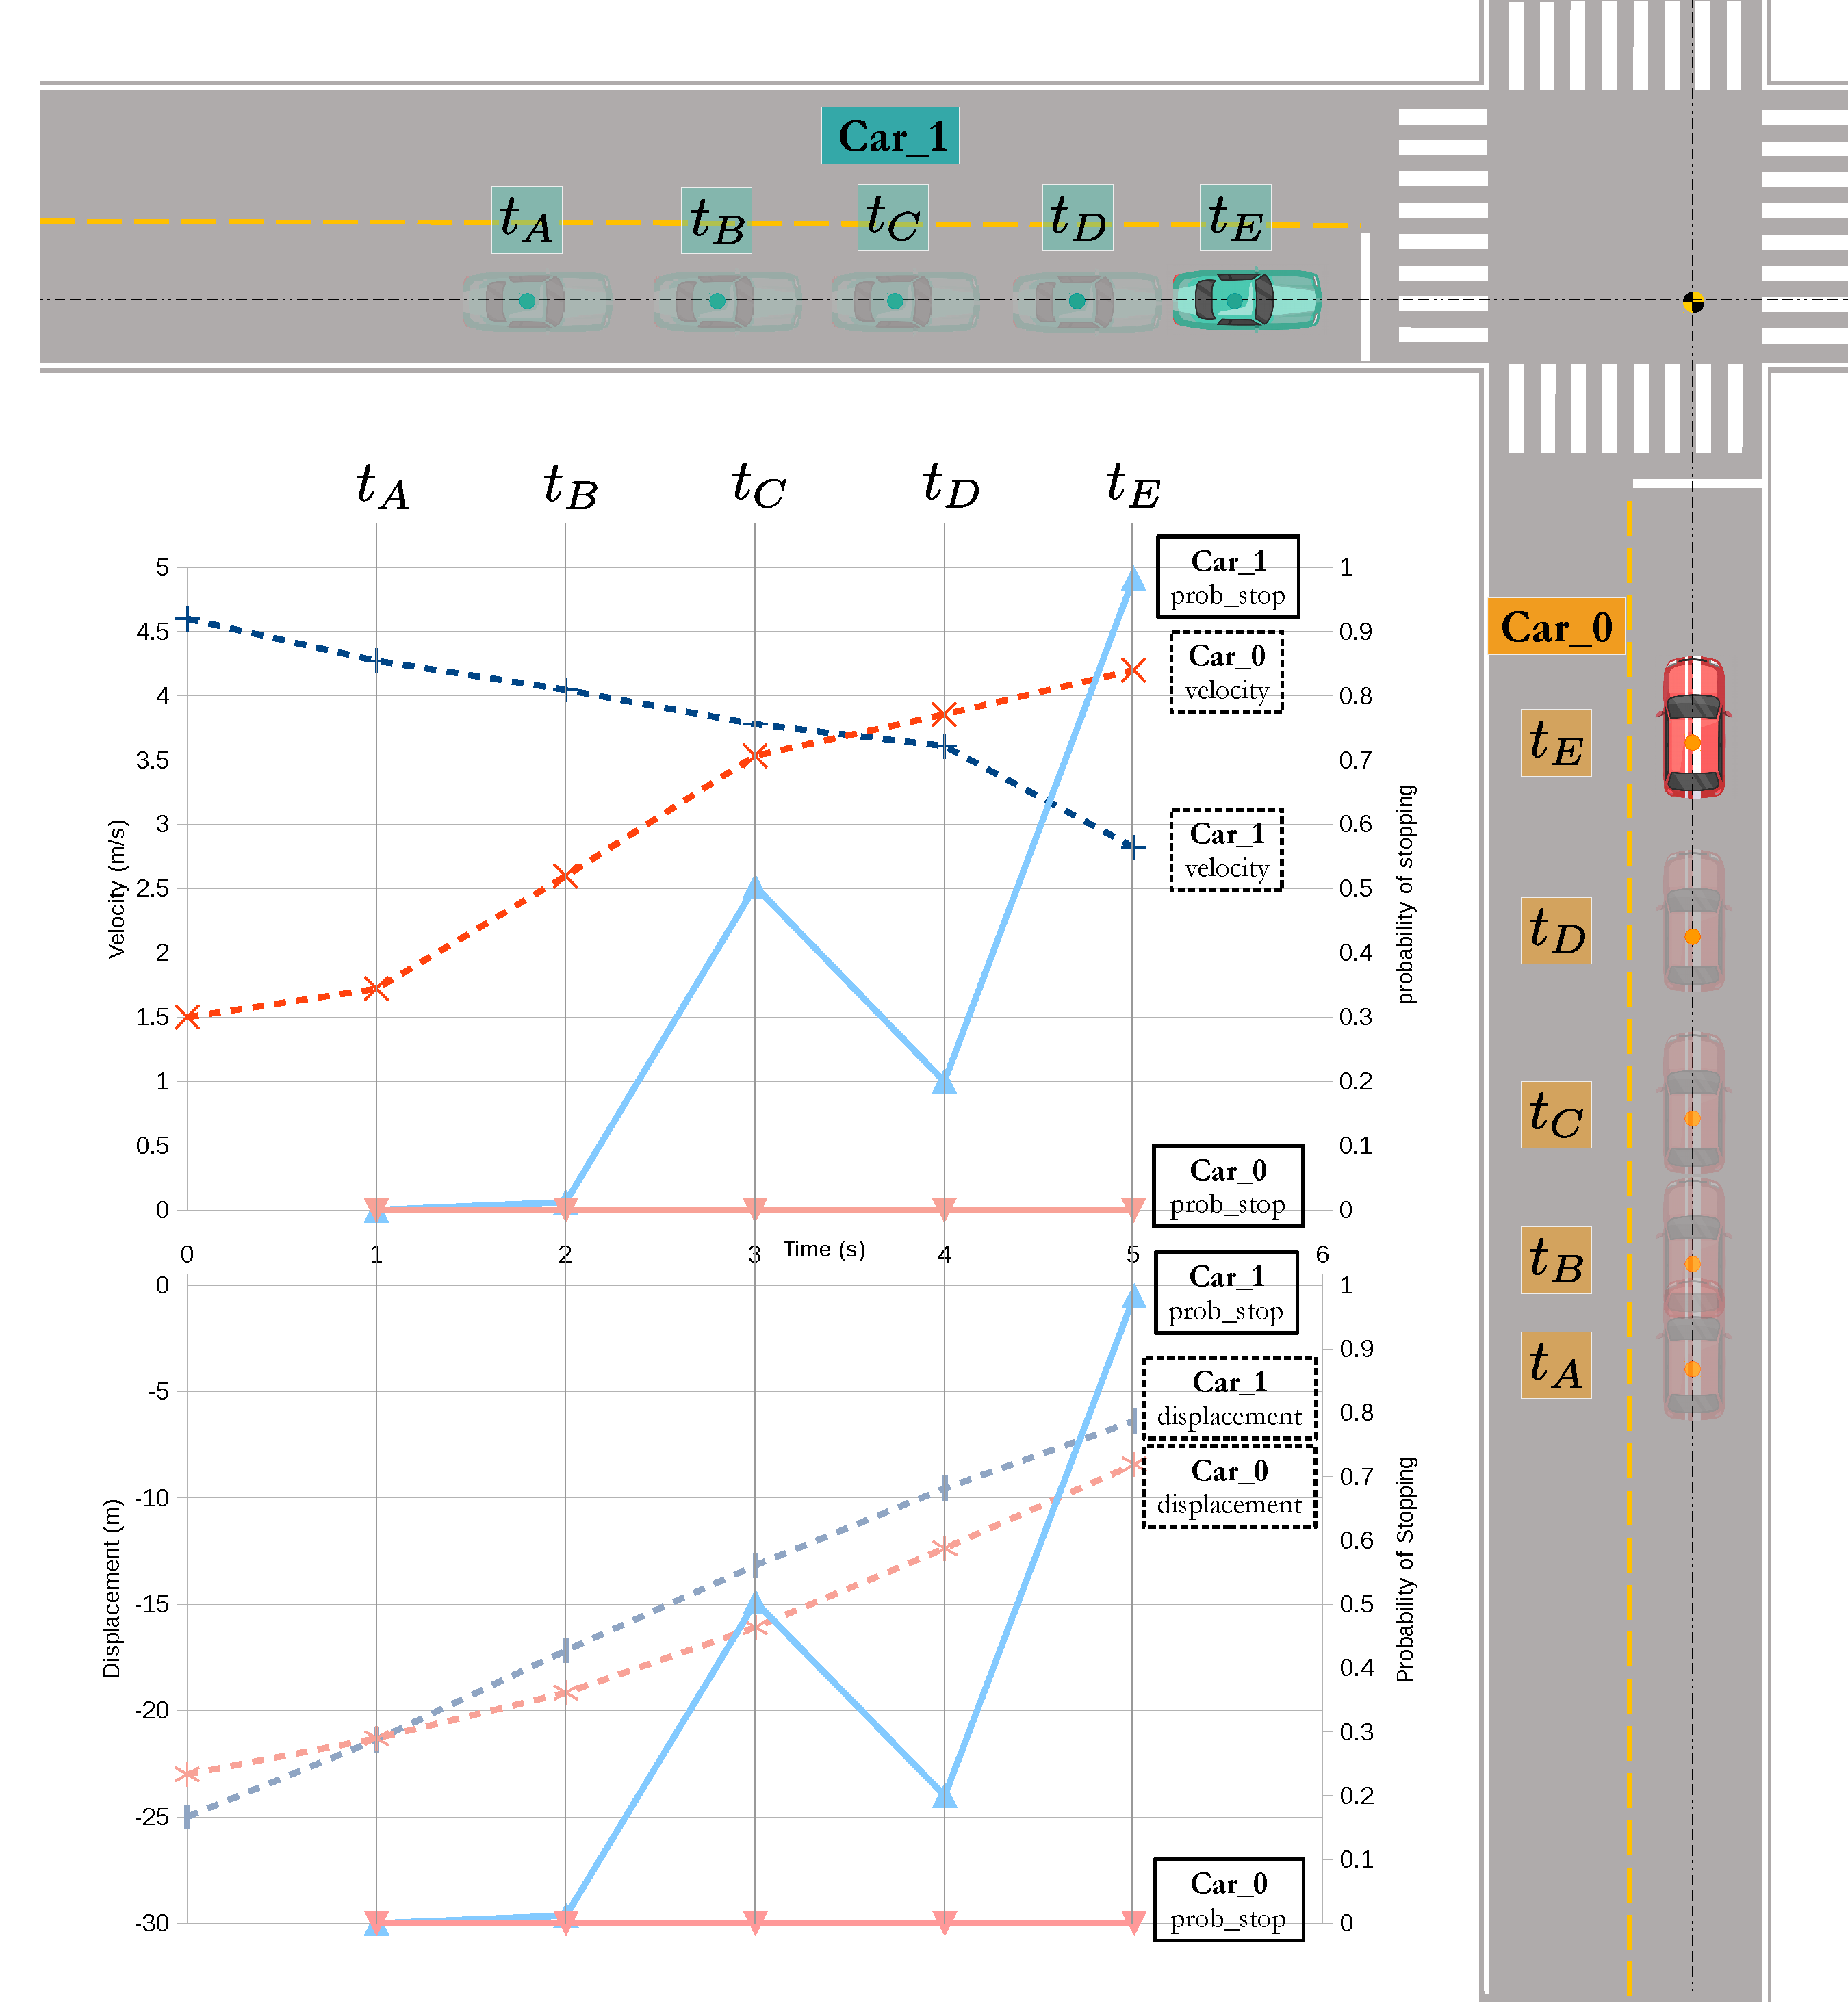
\includegraphics[width=0.4\textwidth]{figure_explaination_1.pdf}
    \label{figure_explaination_1}
    }\hfill
    
    \caption{Illustration of TTC and probability of stopping along with concerning variables.} \label{illustration}
\end{figure}

 
 
In the first case, results of Car\_0 are indicated in shades of red and results of Car\_1 in shades of blue as shown in Fig.~\ref{result_1}. In Fig.~\ref{result_1_TTC} the TTCs of two cars are shown, while in Fig.~\ref{result_1_prob} the velocity versus probability of stopping and displacement versus probability of stopping are shown. Three moments concerning the interactions of Car\_0 and Car\_1 are indicated using grey lines labeled with $t_{A_1}$, $t_{B_1}$ and $t_{C_1}$. 

In the beginning of the event, Car\_0 was slower than Car\_1 and the distances to $\oplus$ for both vehicles were approximately the same. First interaction of two vehicles was indicated by the rising in probability of stopping of Car\_1 occurred at $t_{A_1}$, note that the TTC here is around 4 sec. The rising was due to the shorter distance to $\oplus$ and the deceleration of Car\_1. While Car\_0  was still speeding up, the probability of stopping remained at 0. The probability of stopping of car\_1 raised to almost 85\% near $t_{B_1}$ and 98\% near $t_{C_1}$, as it kept on decelerating with the intention of yielding. At this very moment, if an autonomous vehicle can get access to the probability of stopping of the other agent, it could take advantage of such a high value and speed up to get out of the stand-off situation at the crossroad. However, Car\_0, without knowing the intention of the other traffic participant, chose to slow down and let Car\_1 pass first.  


\begin{figure}[htbp!]
    \centering
    \subfloat[Time to collision.]
    {
    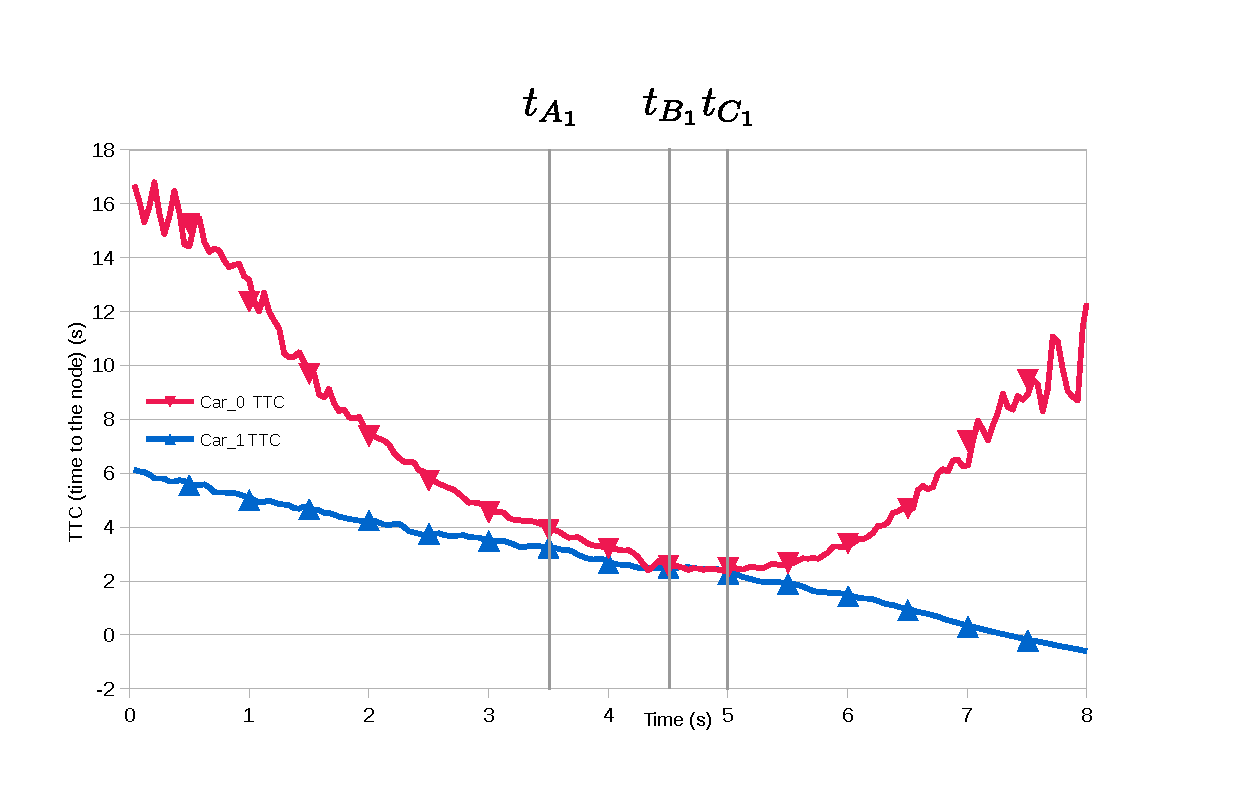
\includegraphics[width=0.49\textwidth]{result_analysis1_TTC.pdf}
    \label{result_1_TTC}
    }\hfill
    \subfloat[Velocity, displacement and probability of stopping.]
    {
    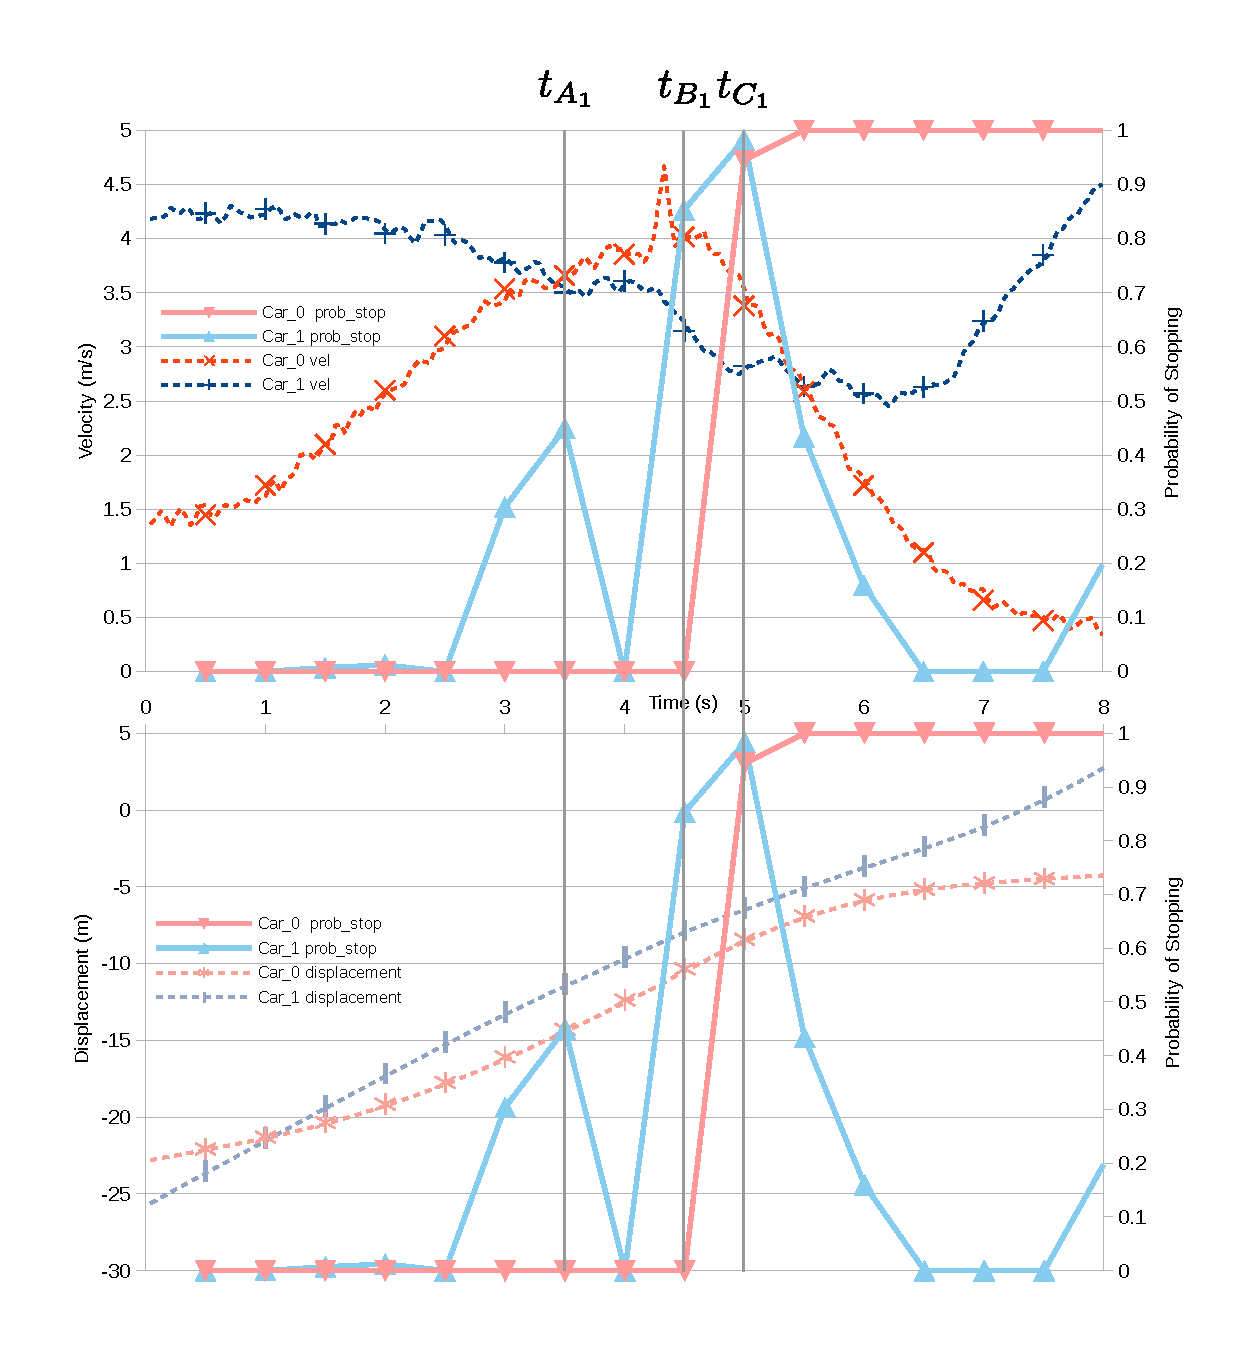
\includegraphics[width=0.49\textwidth]{result_analysis1_prob.pdf}
    \label{result_1_prob}
    }\hfill
    
    \caption{Time to collisioin and probability of stopping along with concerning variables in case I.} \label{result_1}
\end{figure}


In case II, similar situation was shown in Fig.~\ref{result_2}. Note that in this figure, Car\_0 is indicated in shades of blue and Car\_1 in shades of red. In this case, speed of two agents were close with Car\_1 slightly above Car\_0, and Car\_0 is closer to $\oplus$ than Car\_1. Spikes at $t_{A_2}$ for Car\_0 and $t_{B_2}$ for Car\_1 were due to the approaching to $\oplus$ that cause the TTCs drop near the calculated actual TTA and give rise to the rise of the probability of stopping. At $t_{B_2}$, the probability of stopping for Car\_1 rise even higher as a consequence of the deceleration. At $t_{C_2}$, Car\_0 brake drastically at such a small TTC, causing the probability of stopping rise to almost 100\%. In this case, both Car\_0 and Car\_1 could have gotten out of the stand-off at the crossroad, if they know the probability of stopping.


\begin{figure}[htbp!]
    \centering
    \subfloat[Time to collision.]
    {
    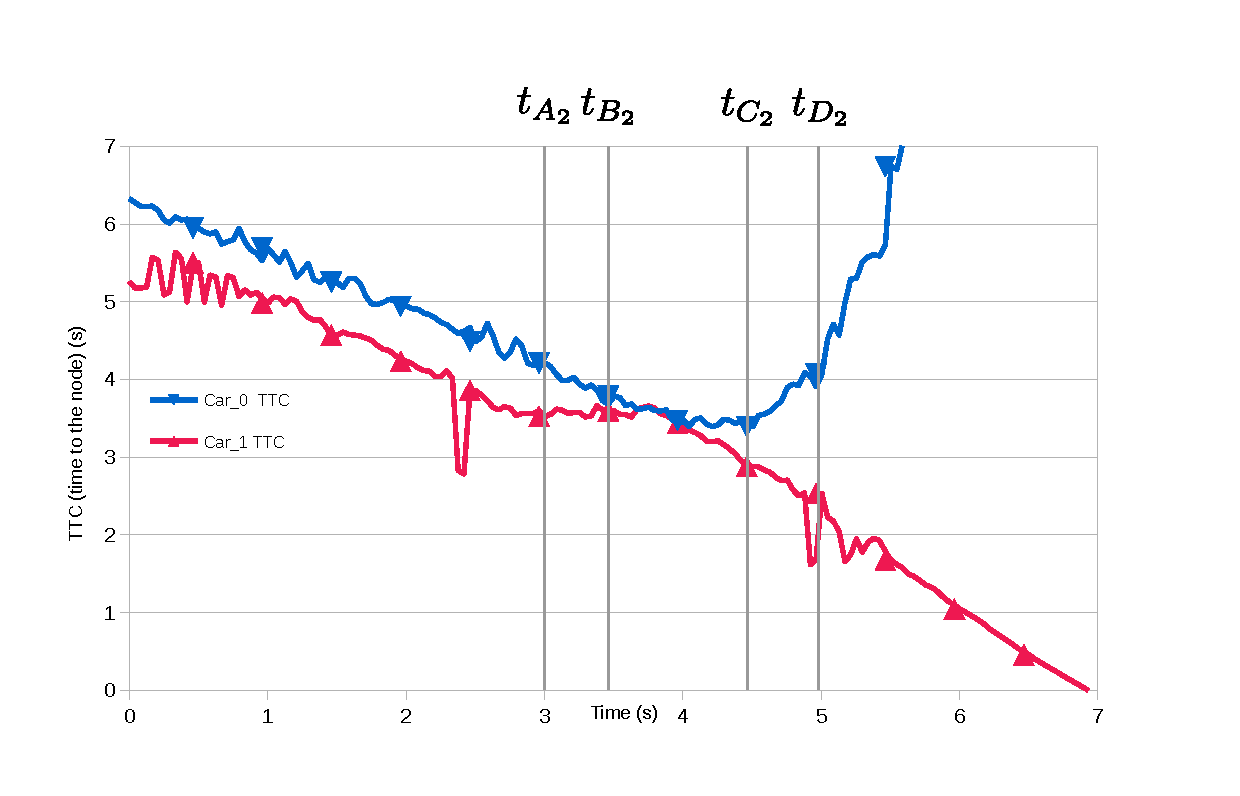
\includegraphics[width=0.49\textwidth]{result_analysis2_TTC.pdf}
    \label{result_2_TTC}
    }\hfill
    \subfloat[Velocity, displacement and probability of stopping.]
    {
    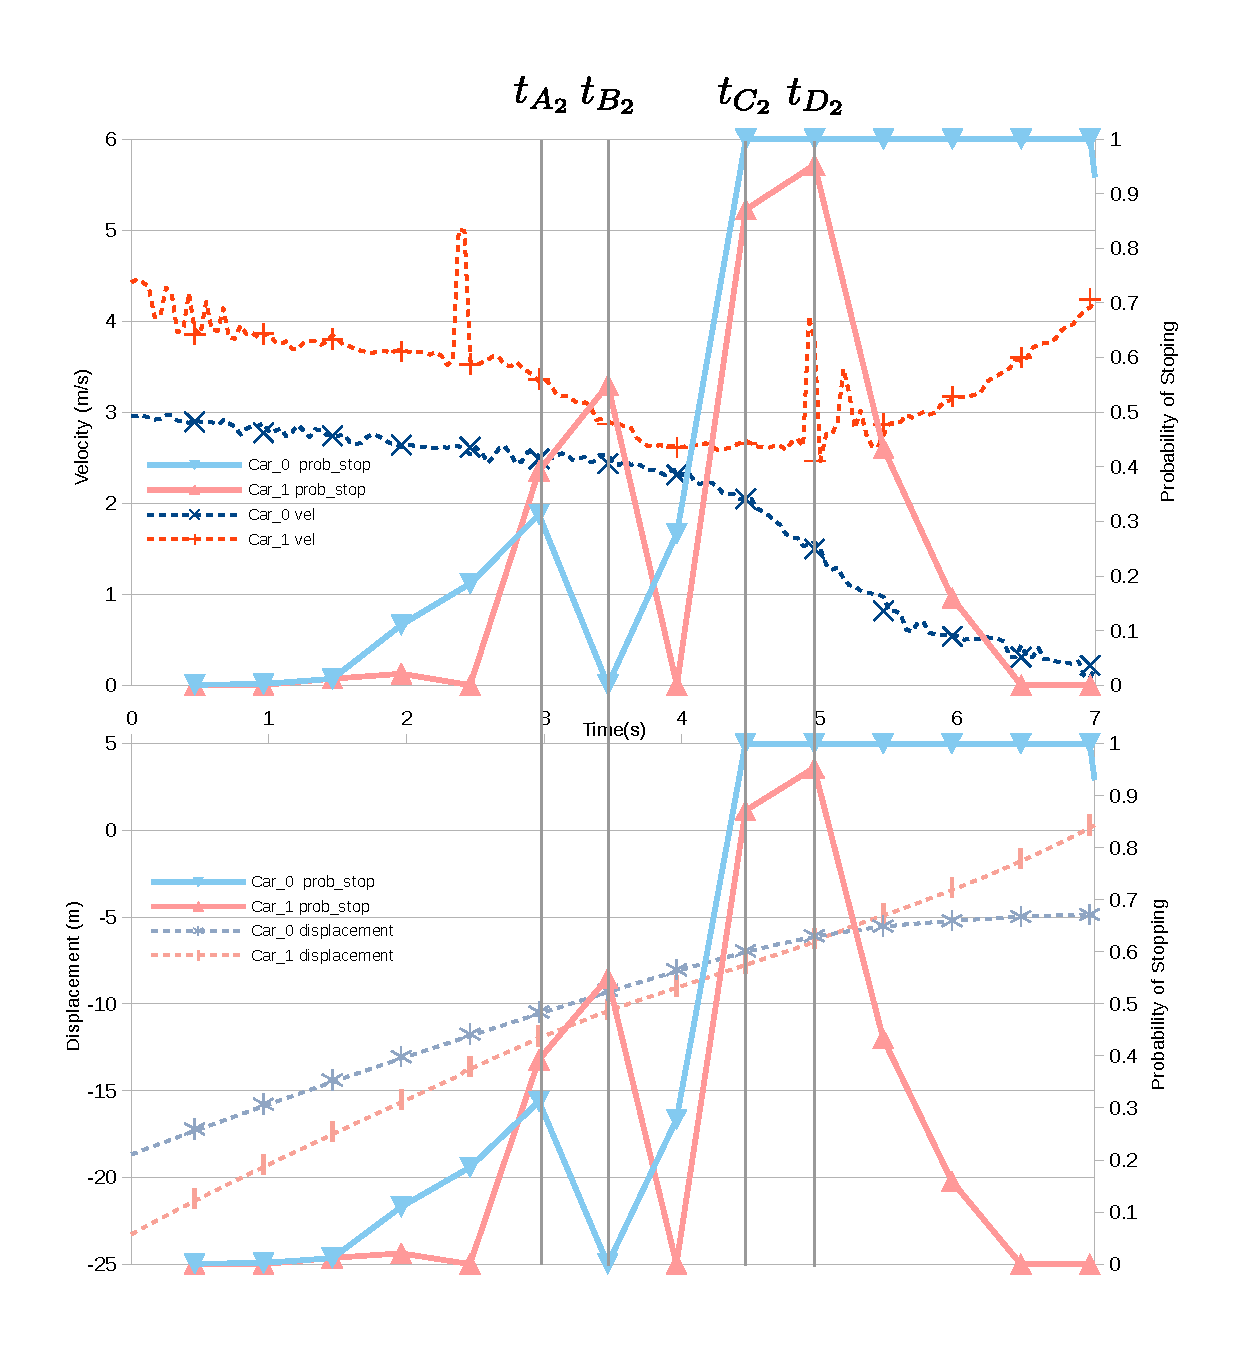
\includegraphics[width=0.49\textwidth]{result_analysis2_prob.pdf}
    \label{result_2_prob}
    }\hfill
    
    \caption{Time to collisioin and probability of stopping along with concerning variables in case II.} \label{result_2}
\end{figure}

To conclude, both cases show similar probabilistic pattern during the observation which is also comparable to human drivers' prediction. Faster vehicles or vehicles closer to $\oplus$ (the intersection of the crossroad) are in dominance of crossing over. From these two cases, we manage to turned the decisions of human drivers into some probabilistic values, which can be perceived by autonomous vehicles.  

In this section, observation of driver behavior at the unsignalized crossroad was conducted. The proposed model can provide the judgements needed for autonomous vehicles to cross over, which is also similar to those of human drivers by the combined evaluation of distance, speed and time. 

%%%%%%%%%%%%%%%%%%%%%%%%%%%%%%%%%%%%%%%%%%%%%%%%%%%%%%%%%%%%%%%%%%%%%%%%
\section{DISCUSSIONS AND CONCLUSIONS}

The acquisition of the probability of stopping requires the use of general distribution of TTA, which is not yet been found in the literature. In this work, we use the critical warning distance in Eqn.~(\ref{TTA_est}) as the variable to estimate the average TTA value. And the estimation error is also considered, as described in Eqn.~(\ref{TTA_mean}). Then, the generated average model for TTA is used to determine the cumulative probability. What is exciting is that, with this assumption, we can also come up with TTA distributions made specifically for people with different characteristics. As mentioned before, a young guy with a Porsche 991 should have a smaller mean and standard deviation for his TTA distribution than an old man with a TOYOTA prius. 

In other words, if we know how the decision is usually been made by the driver, it is more likely that we can predict his or her behavior. It is the same to the parameters which could potentially define the driving pattern of the driver. If a set of well defined parameters of the driver is known, we can then use Eqn.~(\ref{TTA_est}) and (\ref{TTA_mean}) to generate a precise TTA distribution to estimate the chance of braking at some TTC of that driver. As for the reward ratio $\alpha$, as mentioned before, we chose 1.5 in order to have higher probabilities for more obvious results. Even though a more thoroughly evaluated reward ratio might generate more precise results, the trends are still identical. To make these parameters well defined, more observation including details such as age, gender, occupation, etc. should be performed. However, data concerning psychology such as personal traits is usually sensitive to experiments conducted. 

Apart from the parameters selection, the issue regarding sensor errors is also a neglected factor affecting the performance of the model. Nevertheless, with the probabilistic modeling approach used in this paper, it could be easily added. 

At last, this method is also short of validation methods. However, a simulation environment is on the way. We are now building a simulated crossroads using a 2D mobile robot simulator called STAGE. As shown in Fig.~\ref{stage}, we will add the proposed model onto this platform and use the simulated autonomous vehicle to interact with human driver (player) shortly. After that, the evaluation shall be conducted and compared to other methods proposed in the literature.  


\begin{figure}[htbp!]
\begin{center}
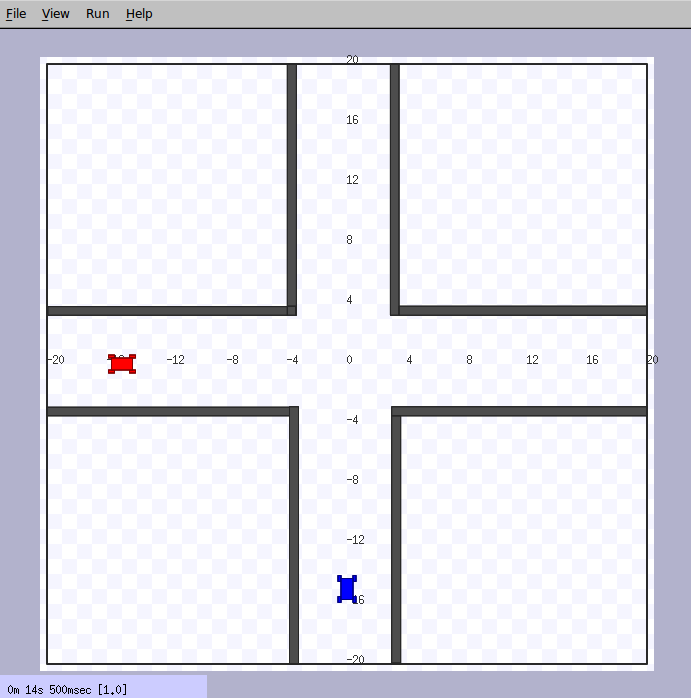
\includegraphics[scale=0.28]{stage.png}
\end{center}
\caption{Simulation environment in STAGE.}
\label{stage} 
\end{figure}

%%%%%%%%%%%%%%%%%%%%%%%%%%%%%%%%%%%%%%%%%%%%%%%%%%%%%%%%%%%%%%%%%%%%%%%%

This work presents a novel model of human driver behaviors that takes relevant variables into account in a probabilistic way and use the result to assess the possibility of that behavior happen. Experiments were conducted with observations at the urban crossroad. The results of the proposed model from two separated cases are consistent and have shown similar judgments as human drivers. However, more works need to be done to evaluate the effectiveness of this model with human drivers at crossroads or in a more complicated urban mixed fleet. Interactive motion planning based on the proposed model could be developed as long as the model is capable of evaluating the uncertainties and be further derived to a higher configuration space. Finally, combine all the above, an autonomous vehicle with the developed motion planning algorithm will then be able to interact with surrounding agents efficiently and safely.

%%%%%%%%%%%%%%%%%%%%%%%%%%%%%%%%%%%%%%%%%%%%%%%%%%%%%%%%%%%%%%%%%%%%%%
\section{Acknowledgements}
This work is partially supported by the Ministry of Science and Technology in Taiwan under grant #MOST 107-2221-E-002 -139. This support is gratefully acknowledged.





% Here's where you specify the bibliography style file.
% The full file name for the bibliography style file 
% used for an ASME paper is asmems4.bst.
%\bibliographystyle{asmems4}
\bibliographystyle{unsrt}
\bibliography{LiuYC_ASME2019_revision}



\end{document}

%%%%%%%%%%%%%%%%%%%%%%%%%%%%%%%%%%%%%%%%%%%%%%%%%%%%%%%%%%%%%%%%%%%%%%%%%%%%%%%%%%%%%%%%%%
%%%%%%%%%%%%%%%%%%%%%%%%%%%%%%%%%%%%%%%%%%%%%%%%%%%%%%%%%%%%%%%%%%%%%%%%%%%%%%%%%%%%%%%%%%
%%%%%%%%%%%%%%%%%%%%%%%%%%%% END OF LIUYC ASME/IDETC 2019 %%%%%%%%%%%%%%%%%%%%%%%%%%%%%%%%
%%%%%%%%%%%%%%%%%%%%%%%%%%%%%%%%%%%%%%%%%%%%%%%%%%%%%%%%%%%%%%%%%%%%%%%%%%%%%%%%%%%%%%%%%%
%%%%%%%%%%%%%%%%%%%%%%%%%%%%%%%%%%%%%%%%%%%%%%%%%%%%%%%%%%%%%%%%%%%%%%%%%%%%%%%%%%%%%%%%%%

